
\section{CKKW parton matching implementation}
\label{sec:monojet_parton_match}

The parton matching techniques are implemented in the mono-jet like MC generation in order to avoid double counting the partons from matrix elements and parton showering. The CKKW matching is better developed and preferred~\cite{Alwall:1405.0301}~\cite{Alwall:0706.2569}. As the illustration sample, the EFT D5 samples are generated with \texttt{MadGraph5\_aMC@NLO} version 2.2.2. The technical implementations are shown as below.

On the generator side, i.e., \texttt{MadGraph5\_aMC@NLO}:
\begin{itemize}
\item \texttt{ickkw = 0}
\item \texttt{ktdurham = }matching scale
\item \texttt{dparameter = 0.4}
\item \texttt{dokt = T}
\item \texttt{ptj=20}
\item \texttt{drjj=0}
\item \texttt{mmjj=0}
\item \texttt{ptj1min=0}
\end{itemize}
On the parton showering side, i.e., \texttt{Pythia 8}:
\begin{itemize}
\item \texttt{Merging:ktType           = 1}
\item \texttt{Merging:TMS              = }matching scale
\item \texttt{1000022:all = chi chi~ 2 0 0 30.0 0.0 0.0 0.0 0.0}
\item \texttt{1000022:isVisible = false}
\item \texttt{Merging:doKTMerging      = on}
\item \texttt{Merging:Process          = pp>{chi,1000022}{chi~,-1000022}}
\item \texttt{Merging:nJetMax          = 2}
\end{itemize}
The matching scales should be the same for the generation and parton showering. In \texttt{MadGraph5\_aMC@NLO}, the particle data group ID \texttt{1000022} is used for weakly interacting dark matter candidates, which should be informed to \texttt{Pythia 8}. 

In this test we are generating the process with up to two parton emissions, so the command \texttt{Merging:nJetMax = 2} is applied to \texttt{Pythia 8}. The different parton emission cases are generated separately:
\begin{itemize}
\item \texttt{p p > chi chi~}
\item \texttt{p p > chi chi~ j}
\item \texttt{p p > chi chi~ j j}
\end{itemize}
Two matching scales are tested at 30 and 80 GeV. The differential jet rates are shown in Fig. \ref{fig:CKKW_D5_30} for matching scale 30 GeV and Fig. \ref{fig:CKKW_D5_80} for 80 GeV. The 80 GeV matching scale gives smoother distribution, which is desired to avoid artifical effect due to parton matching. There will be a small tink around the matching scale for both cases.

\begin{figure}[h!]
	\centering  
	\subfloat[$1\rightarrow2$ parton process]{%
		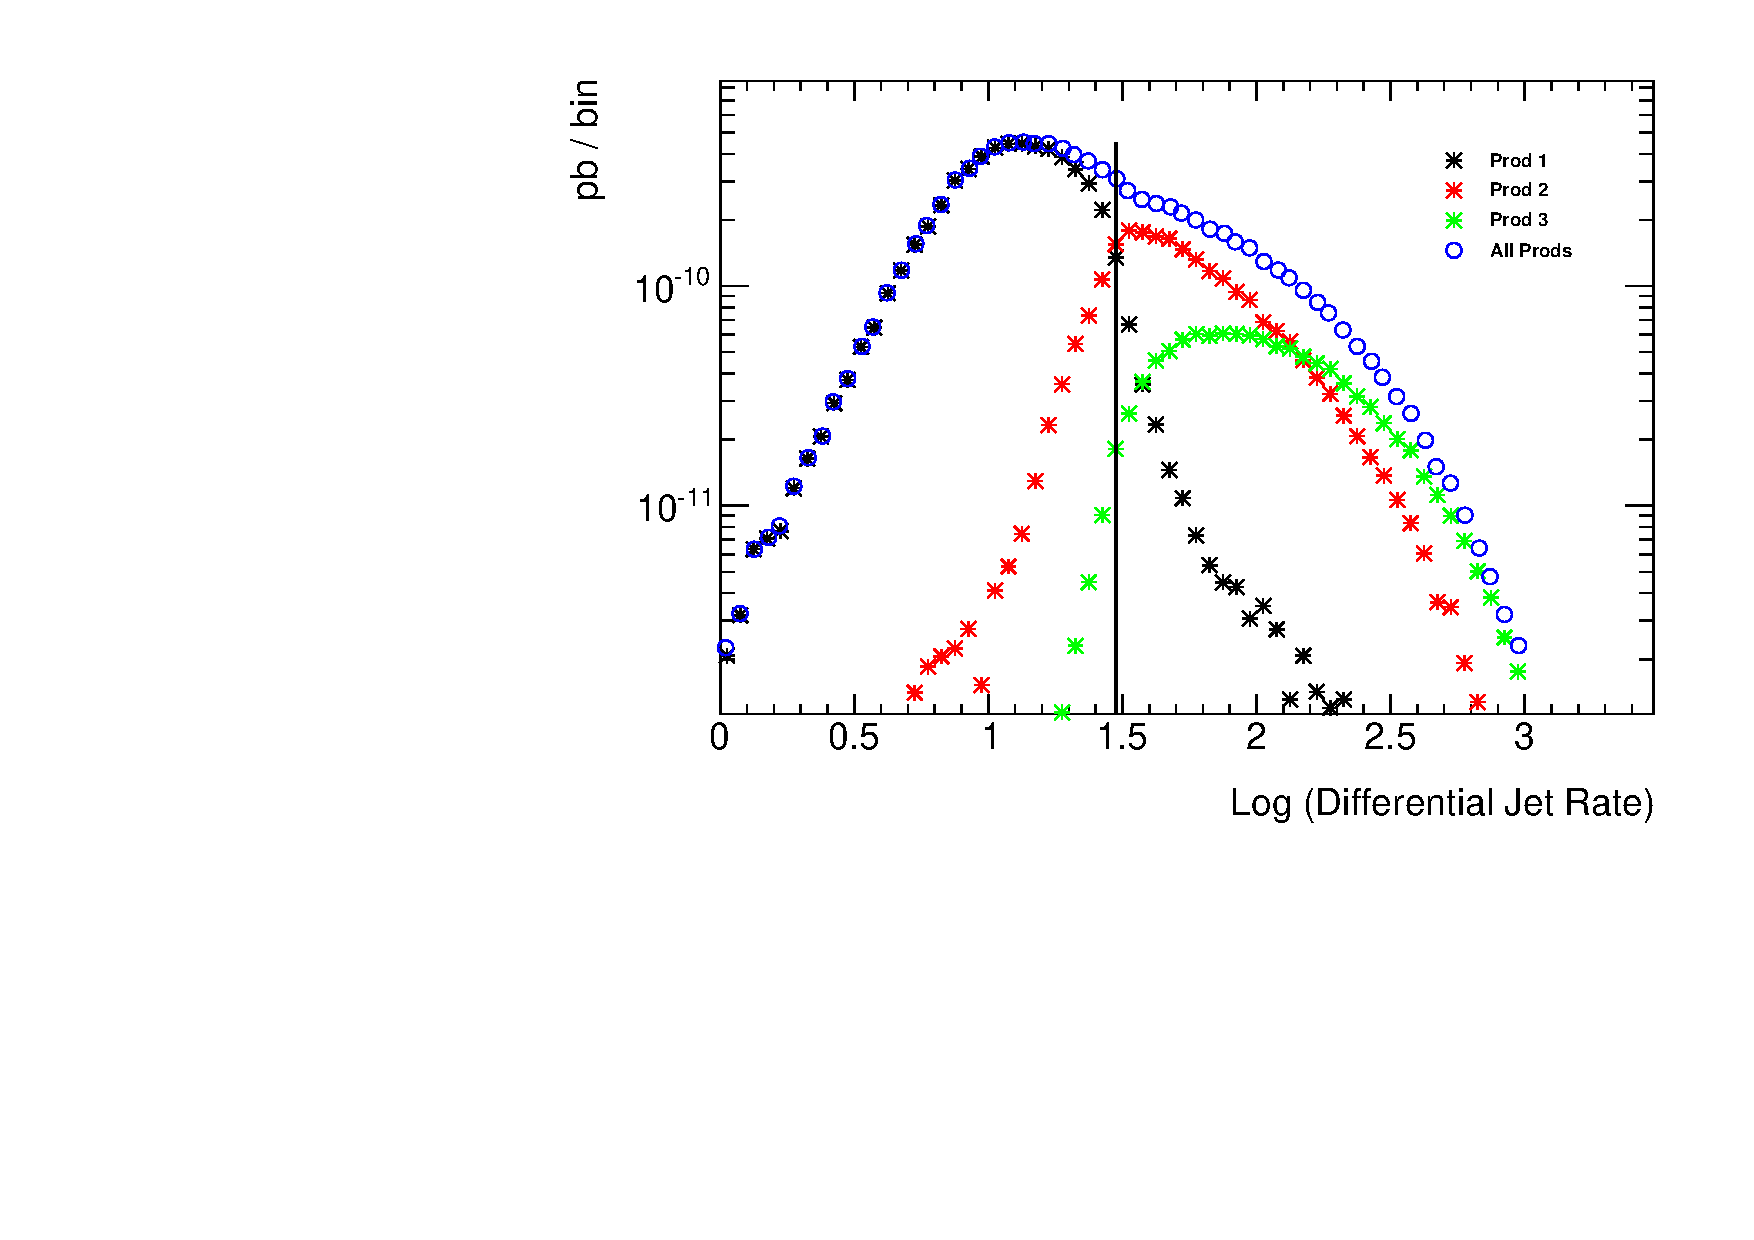
\includegraphics[width=0.48\linewidth]{figures/monojet_appendix/HistoJet1to2_30.pdf}
	}
	\hfill
	\subfloat[$2\rightarrow3$ parton process]{%
		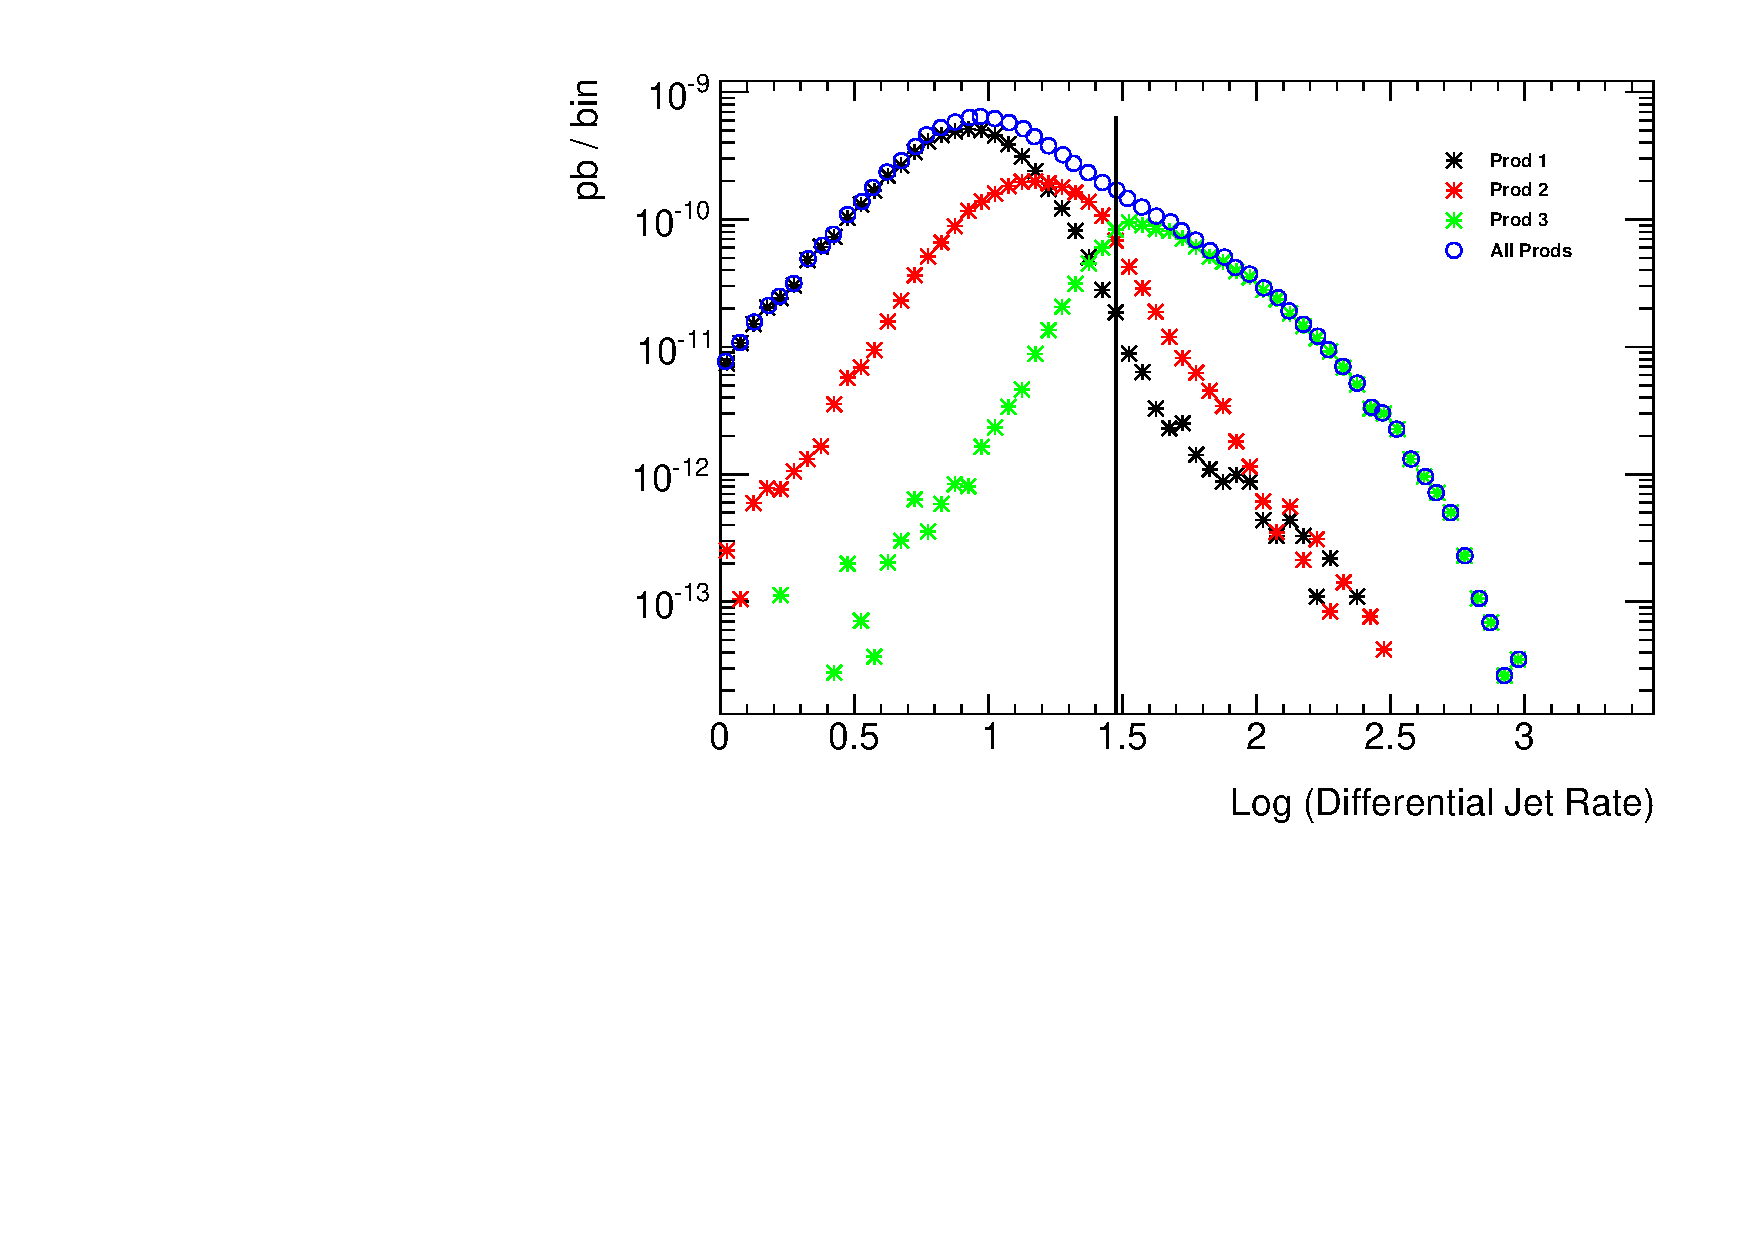
\includegraphics[width=0.48\linewidth]{figures/monojet_appendix/HistoJet2to3_30.pdf}
	}
	\hfill
	\subfloat[$3\rightarrow4$ parton process]{%
		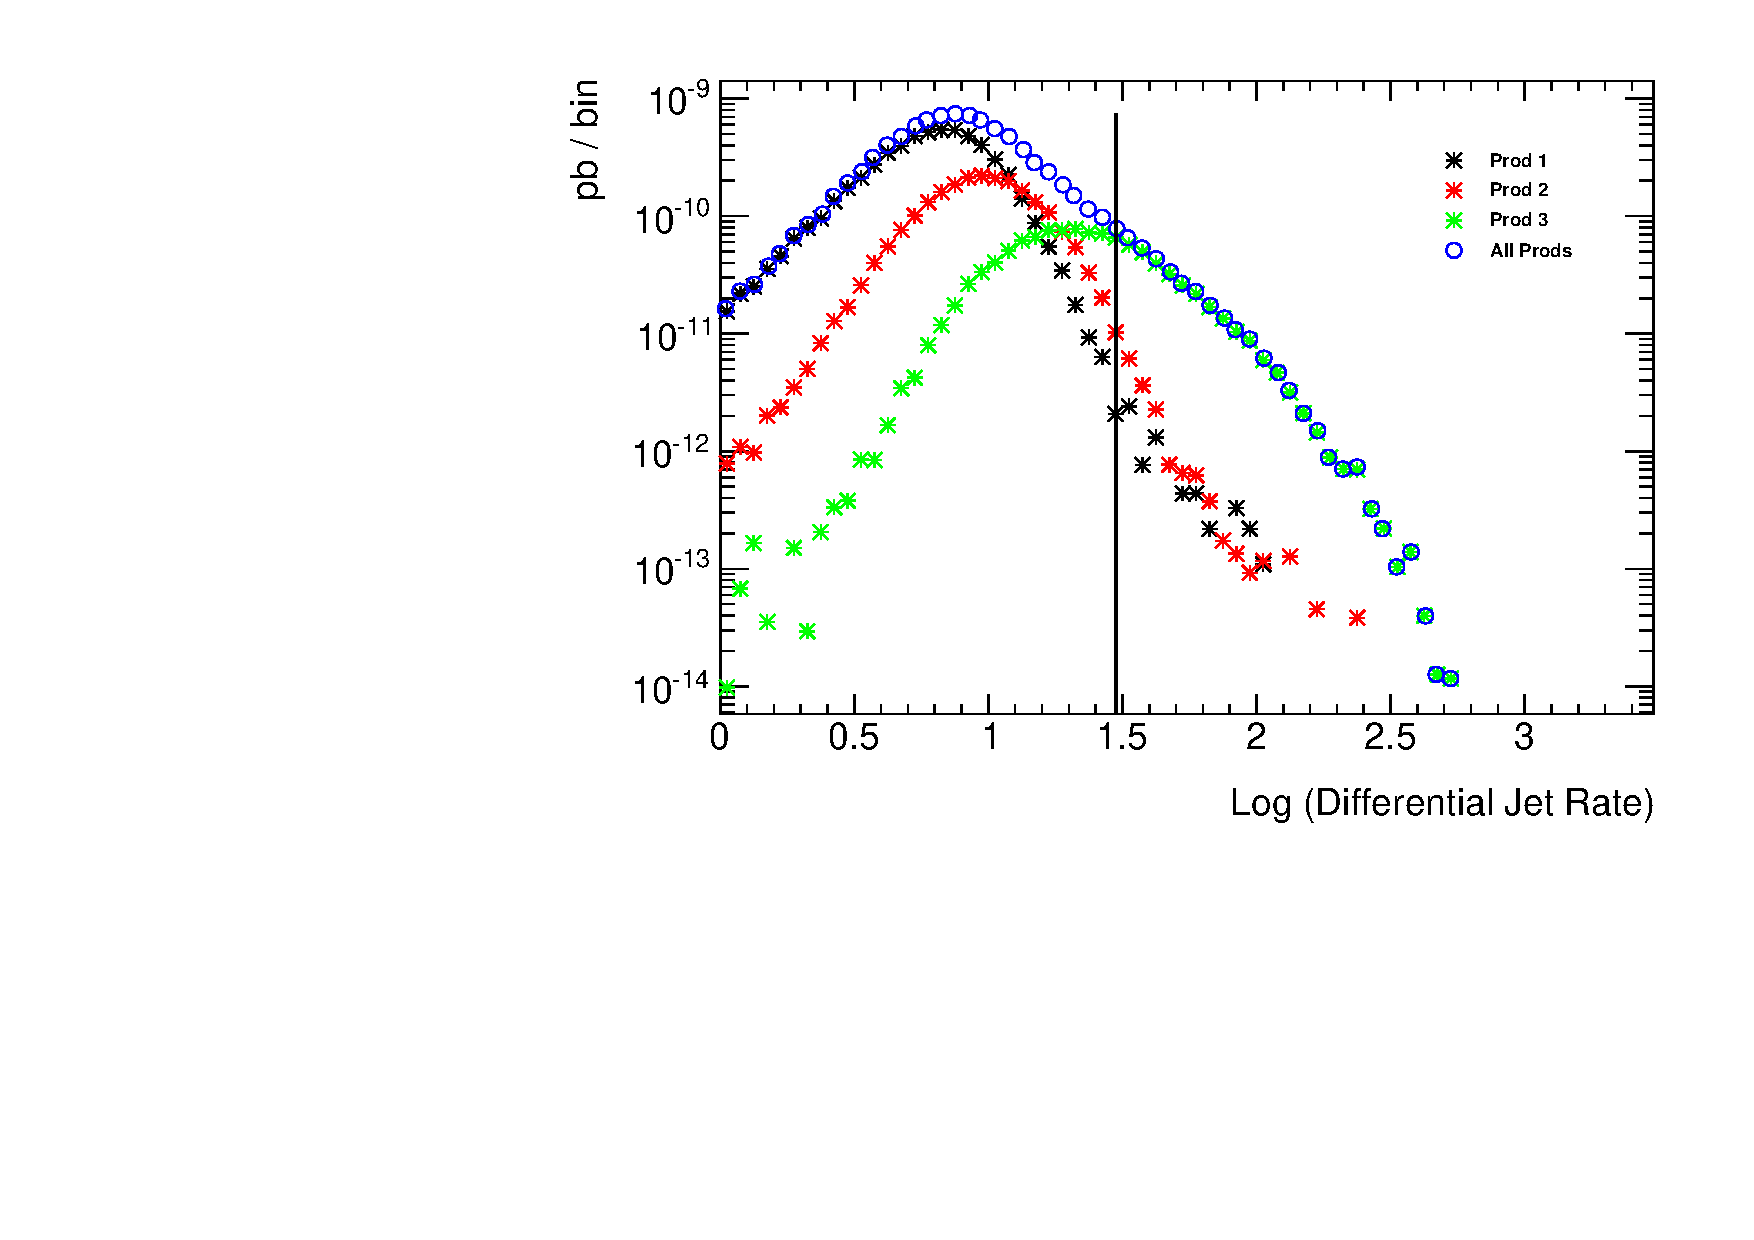
\includegraphics[width=0.48\linewidth]{figures/monojet_appendix/HistoJet3to4_30.pdf}
	}
	\hfill
	\subfloat[$4\rightarrow5$ parton process]{%
		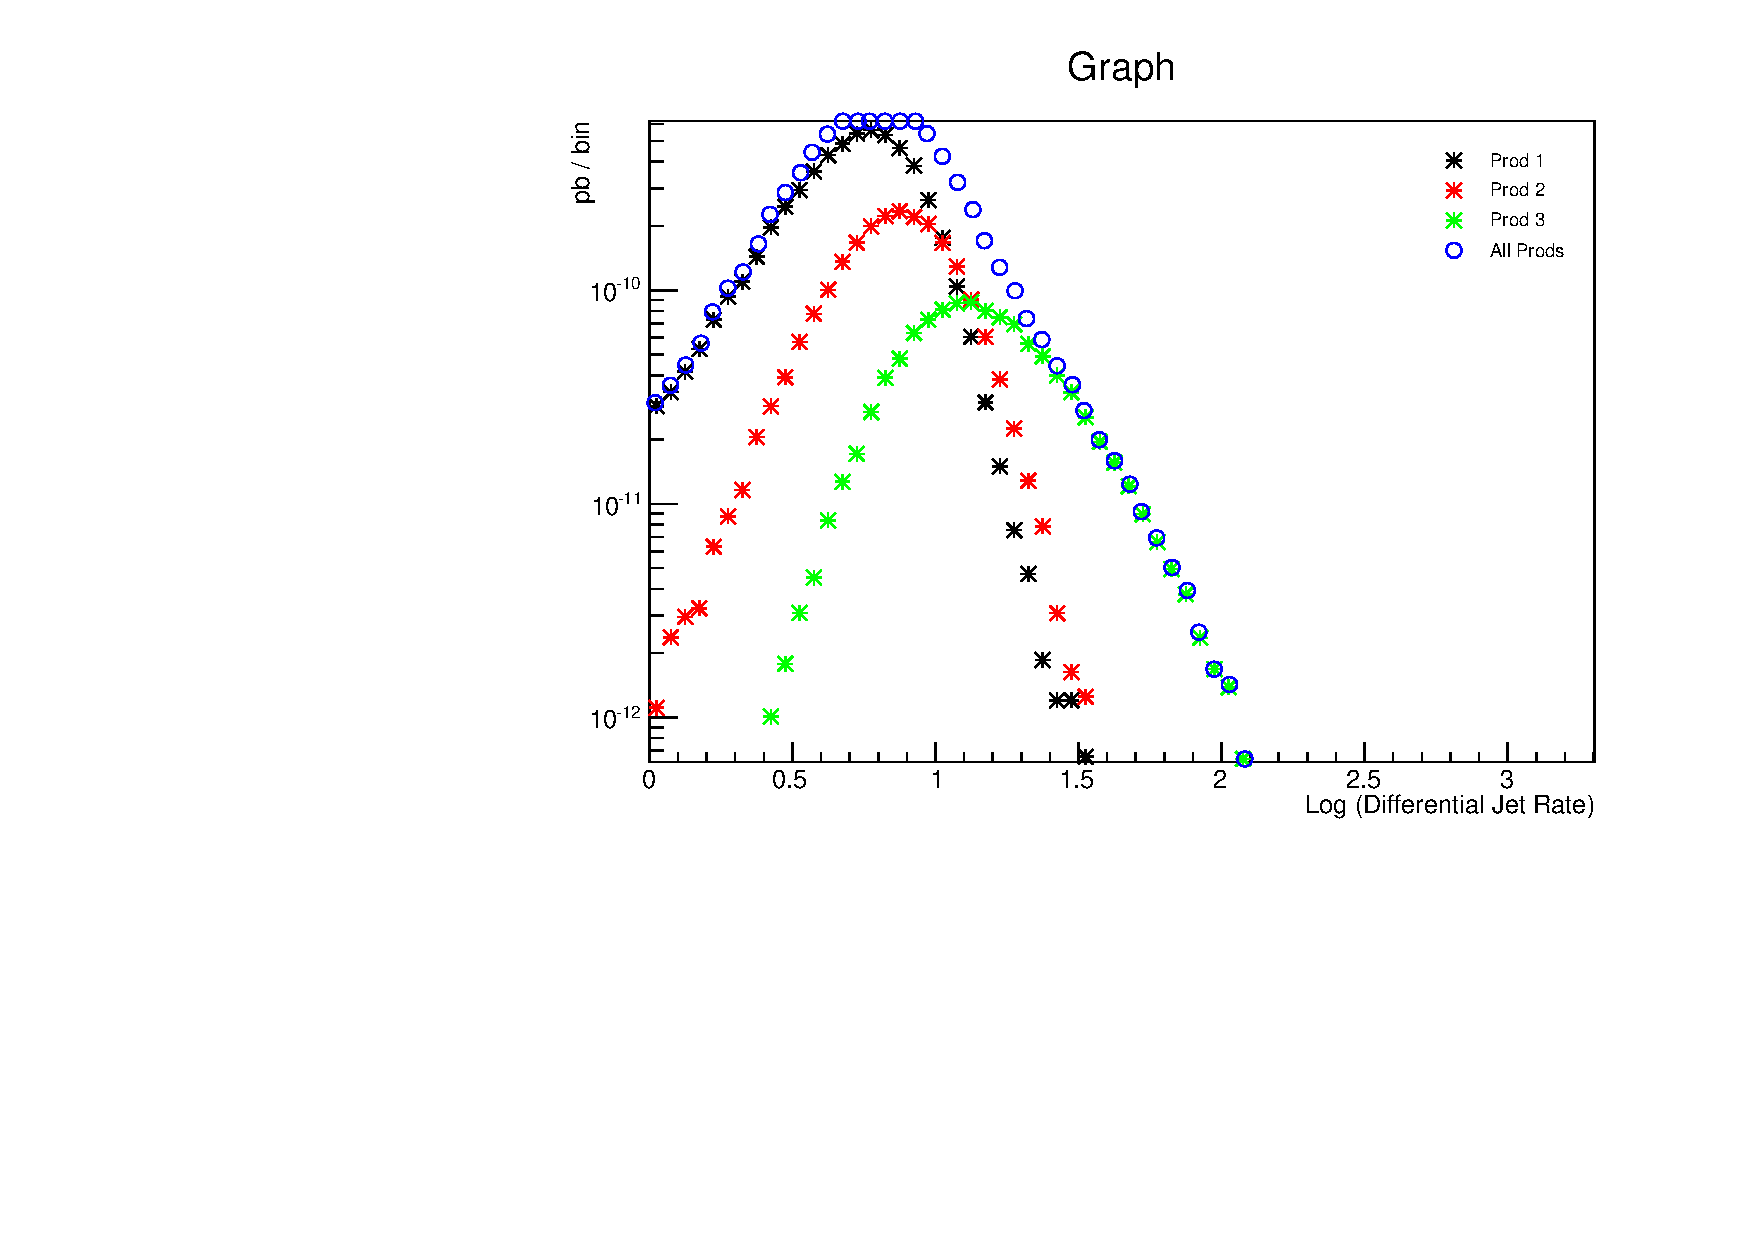
\includegraphics[width=0.48\linewidth]{figures/monojet_appendix/HistoJet4to5_30.pdf}
	}
	\caption{Jet differential rates distributions for EFT D5 sample with CKKW matching scale at 30 GeV. 0-, 1- and 2-parton emission cases are generated separatedly. A vertical line is drawn at the matching scale.}
	\label{fig:CKKW_D5_30}
\end{figure}


\begin{figure}[h!]
	\centering  
	\subfloat[$1\rightarrow2$ parton process]{%
		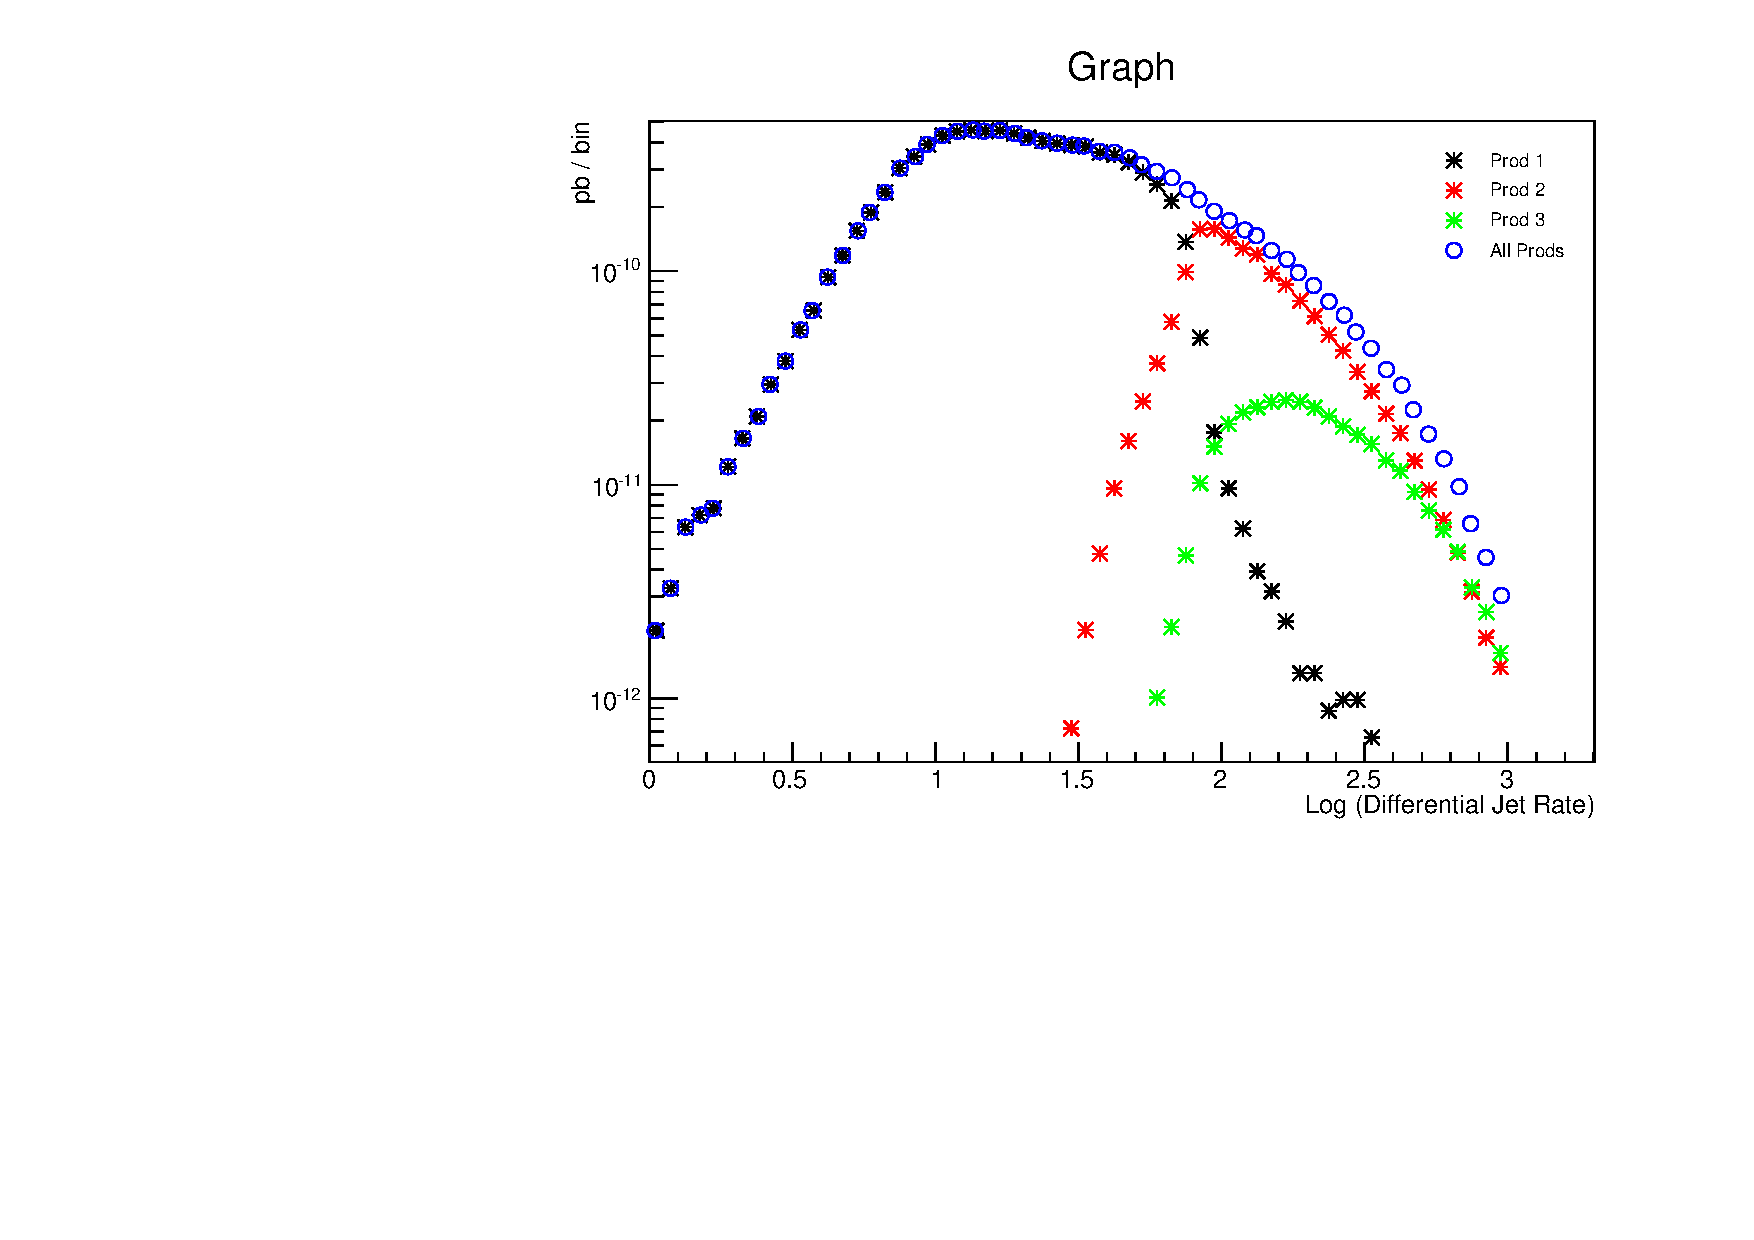
\includegraphics[width=0.48\linewidth]{figures/monojet_appendix/HistoJet1to2_80.pdf}
	}
	\hfill
	\subfloat[$2\rightarrow3$ parton process]{%
		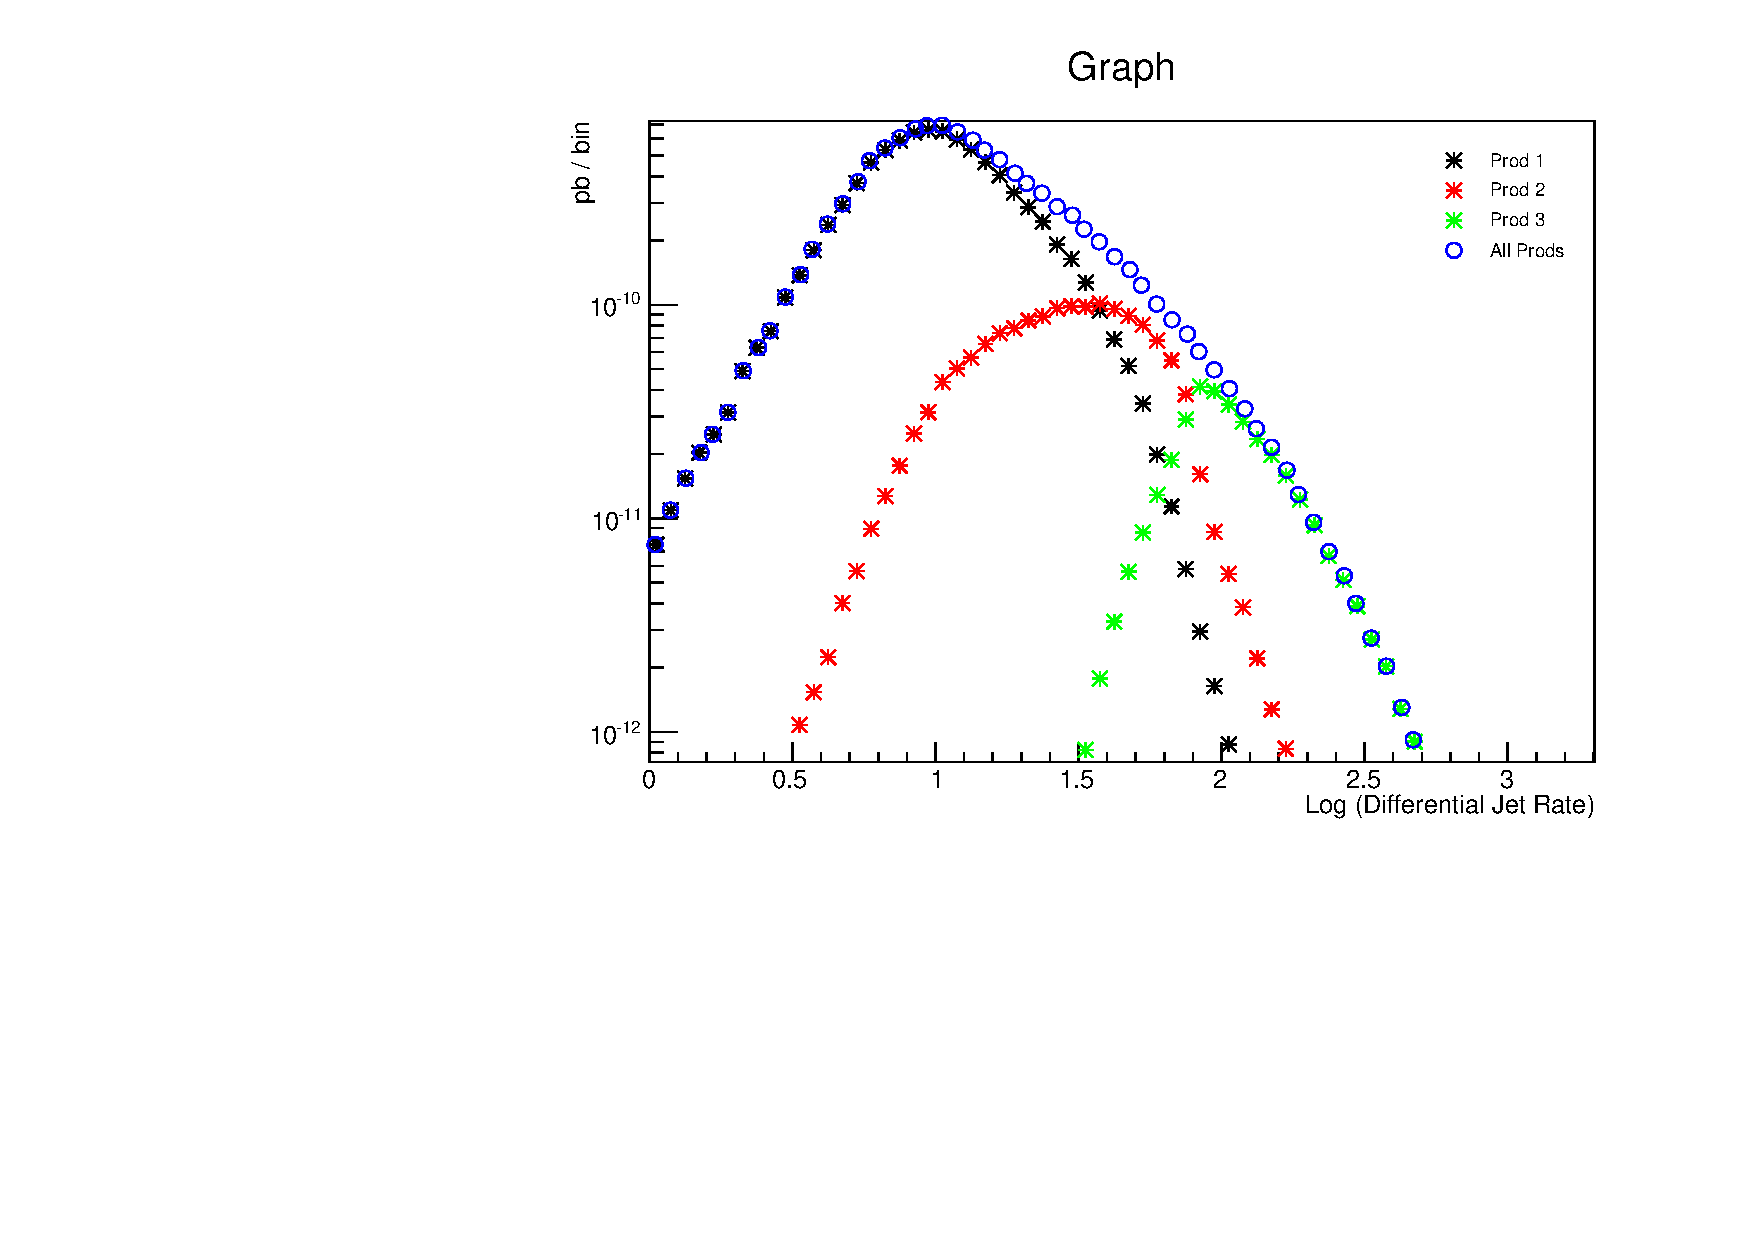
\includegraphics[width=0.48\linewidth]{figures/monojet_appendix/HistoJet2to3_80.pdf}
	}
	\hfill
	\subfloat[$3\rightarrow4$ parton process]{%
    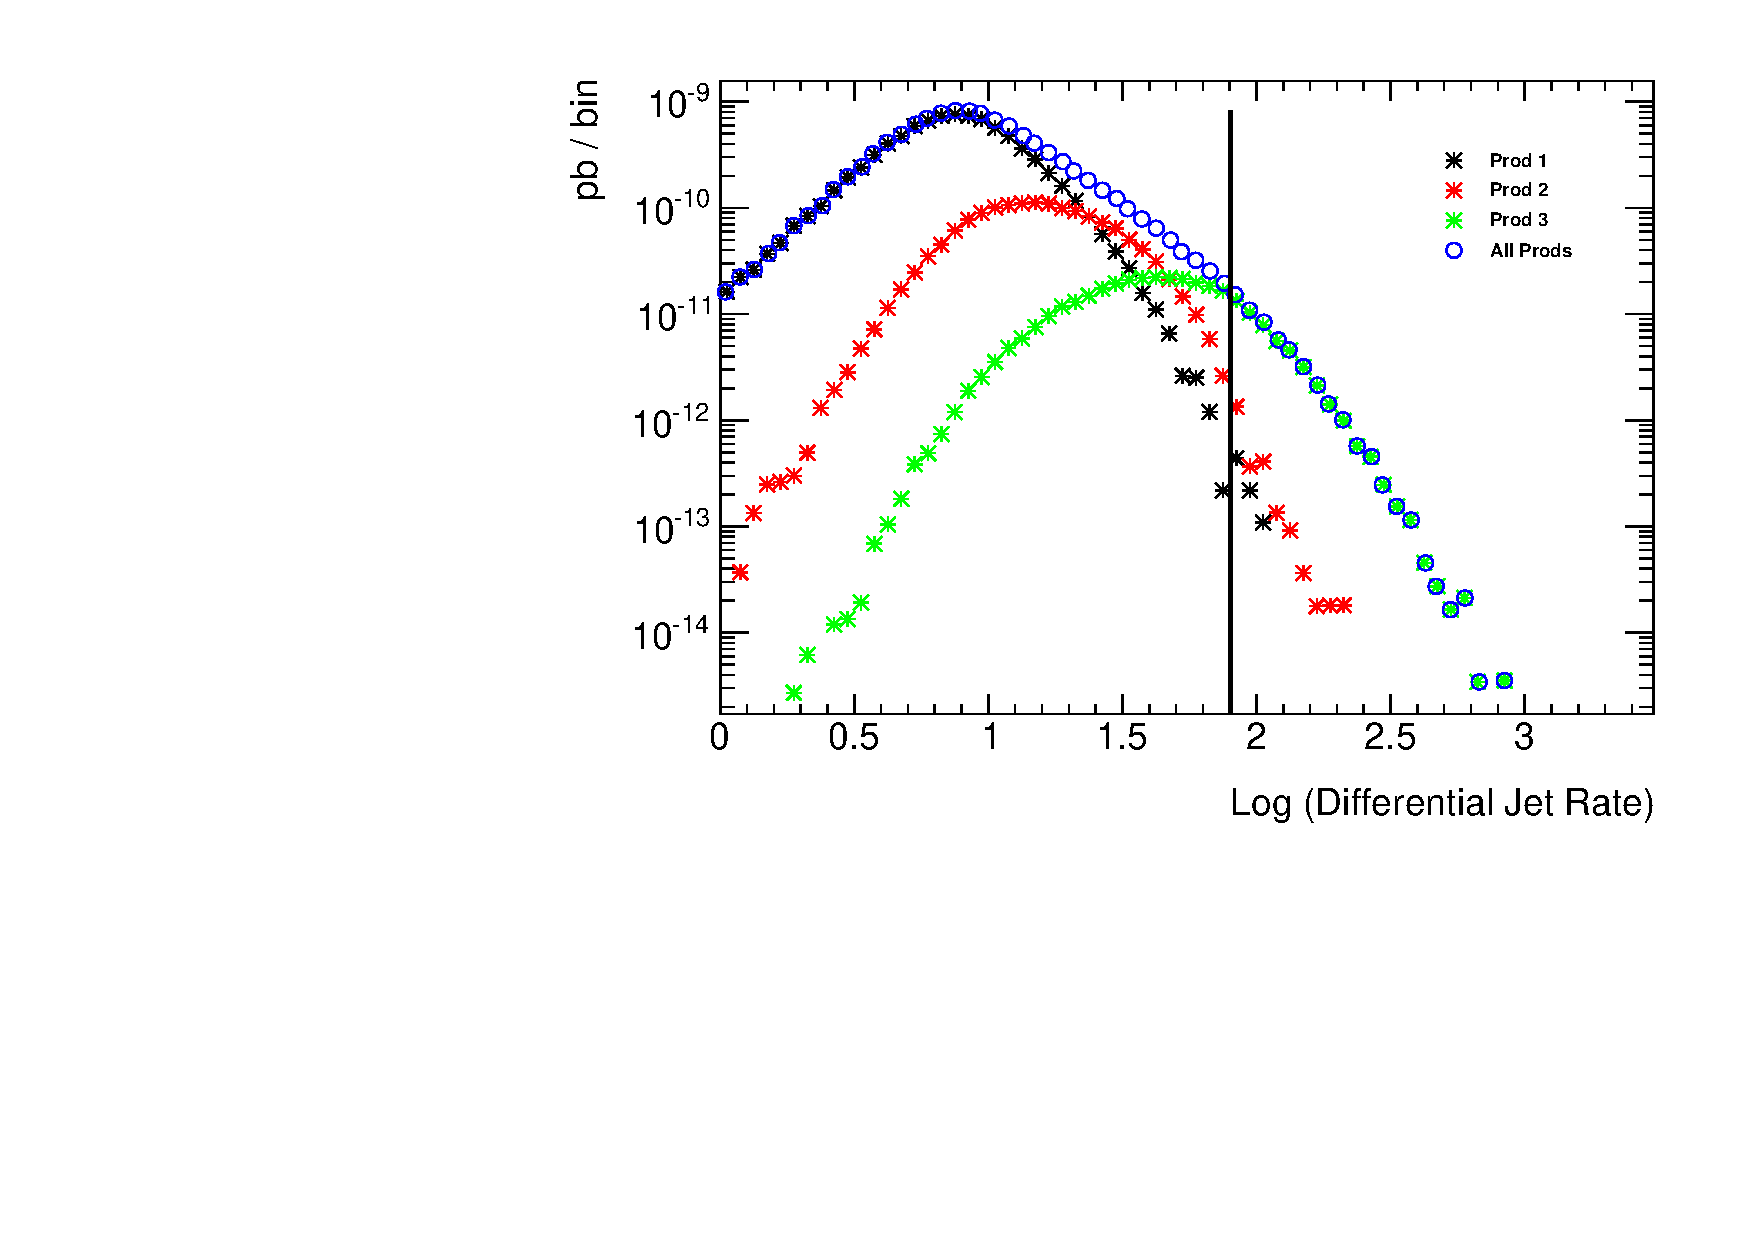
\includegraphics[width=0.48\linewidth]{figures/monojet_appendix/HistoJet3to4_80.pdf}
	}
	\hfill
	\subfloat[$4\rightarrow5$ parton process]{%
    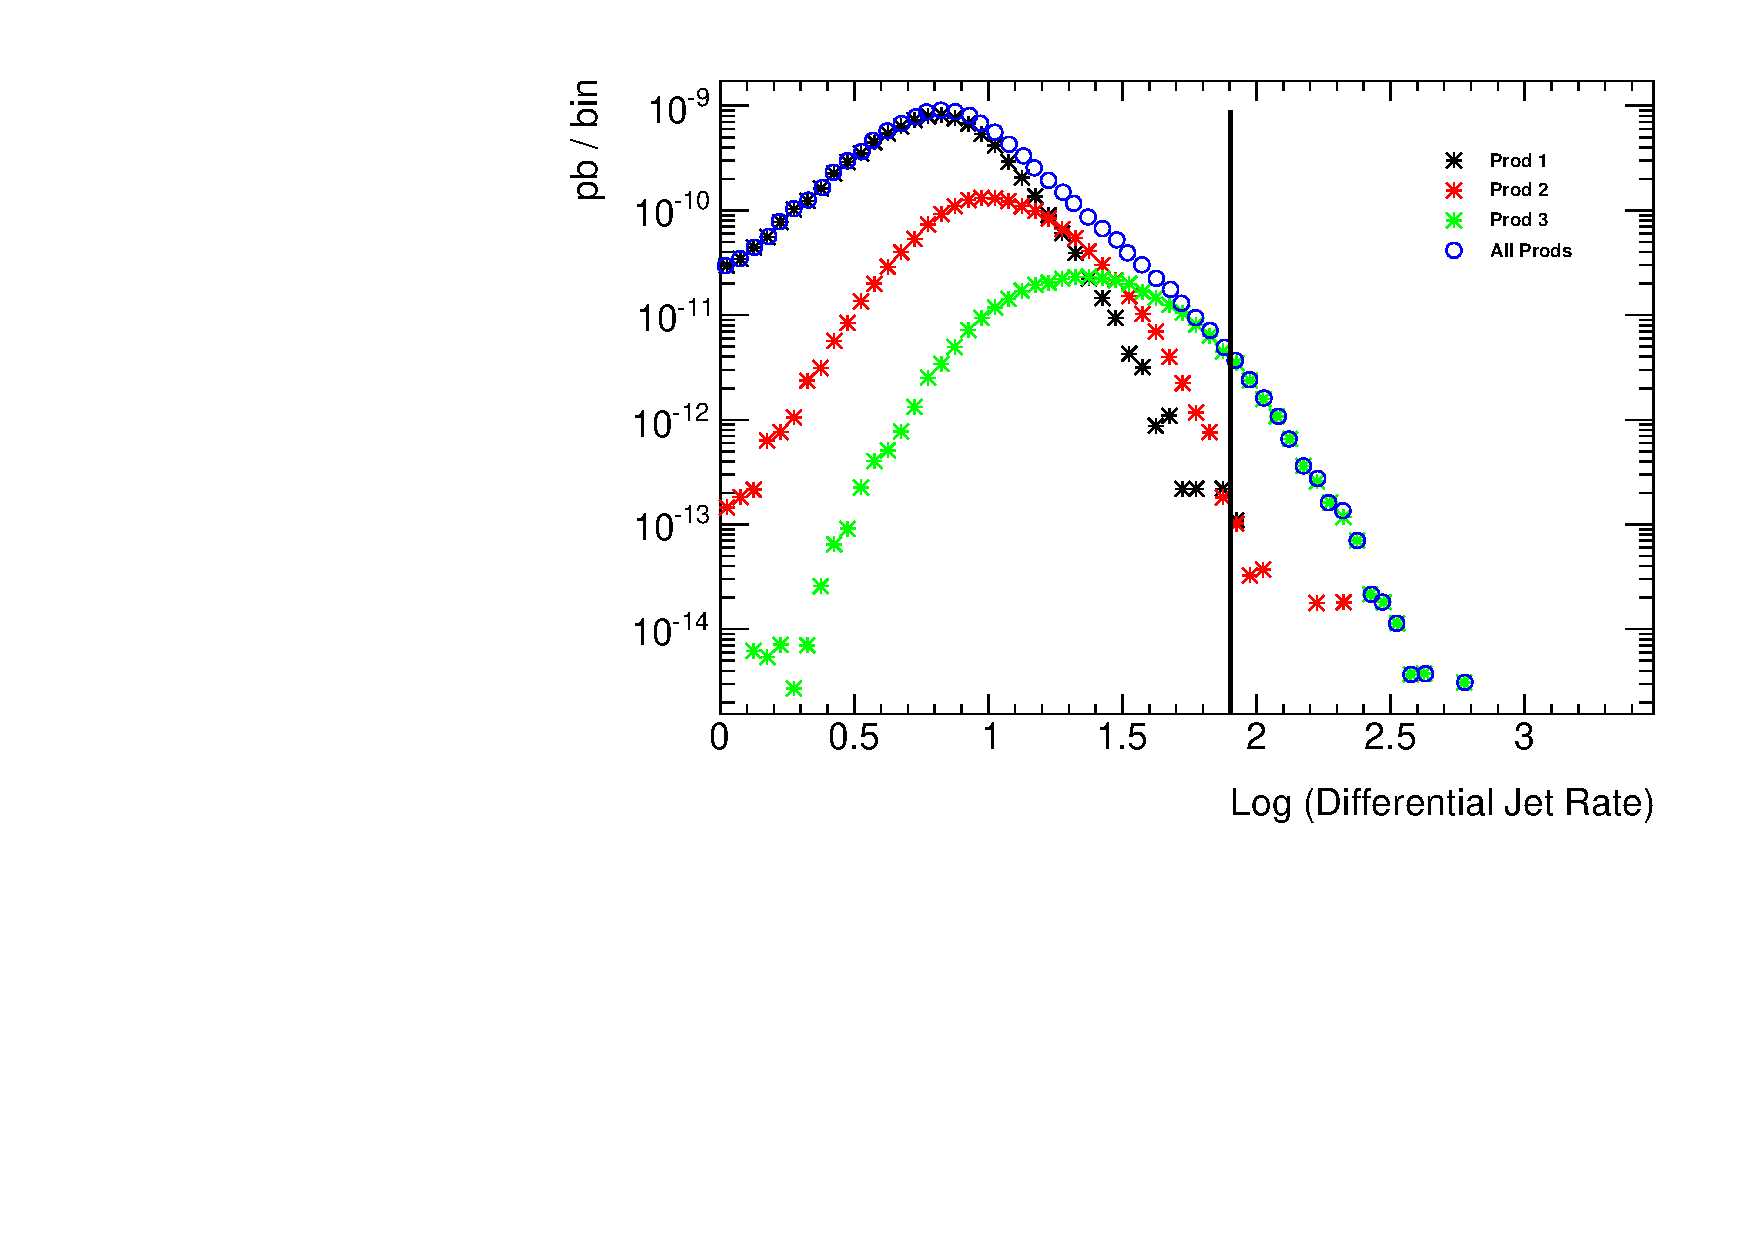
\includegraphics[width=0.48\linewidth]{figures/monojet_appendix/HistoJet4to5_80.pdf}
	}
  \caption{Jet differential rates distributions for EFT D5 sample with CKKW matching scale at 80 GeV. 0-, 1- and 2-parton emission cases are generated separatedly. A vertical line is drawn at the matching scale.}
  \label{fig:CKKW_D5_80}
\end{figure}

To compare the effect in a finer step, the matching scales at 30, 50, 70, 80 and 90 GeV are plotted in Fig\ref{fig:CKKW_D5_zoom}. Globally good agreement is seen among different matching scales, with some difference observed around the matching scale. A closer look in this range shows that the 80 and 90 GeV matching scales produce very close distributions, so it is safe to use 80 GeV as the baseline matching scale.

\begin{figure}[h!]
	\centering  
	\subfloat[$1\rightarrow2$ parton process]{%
		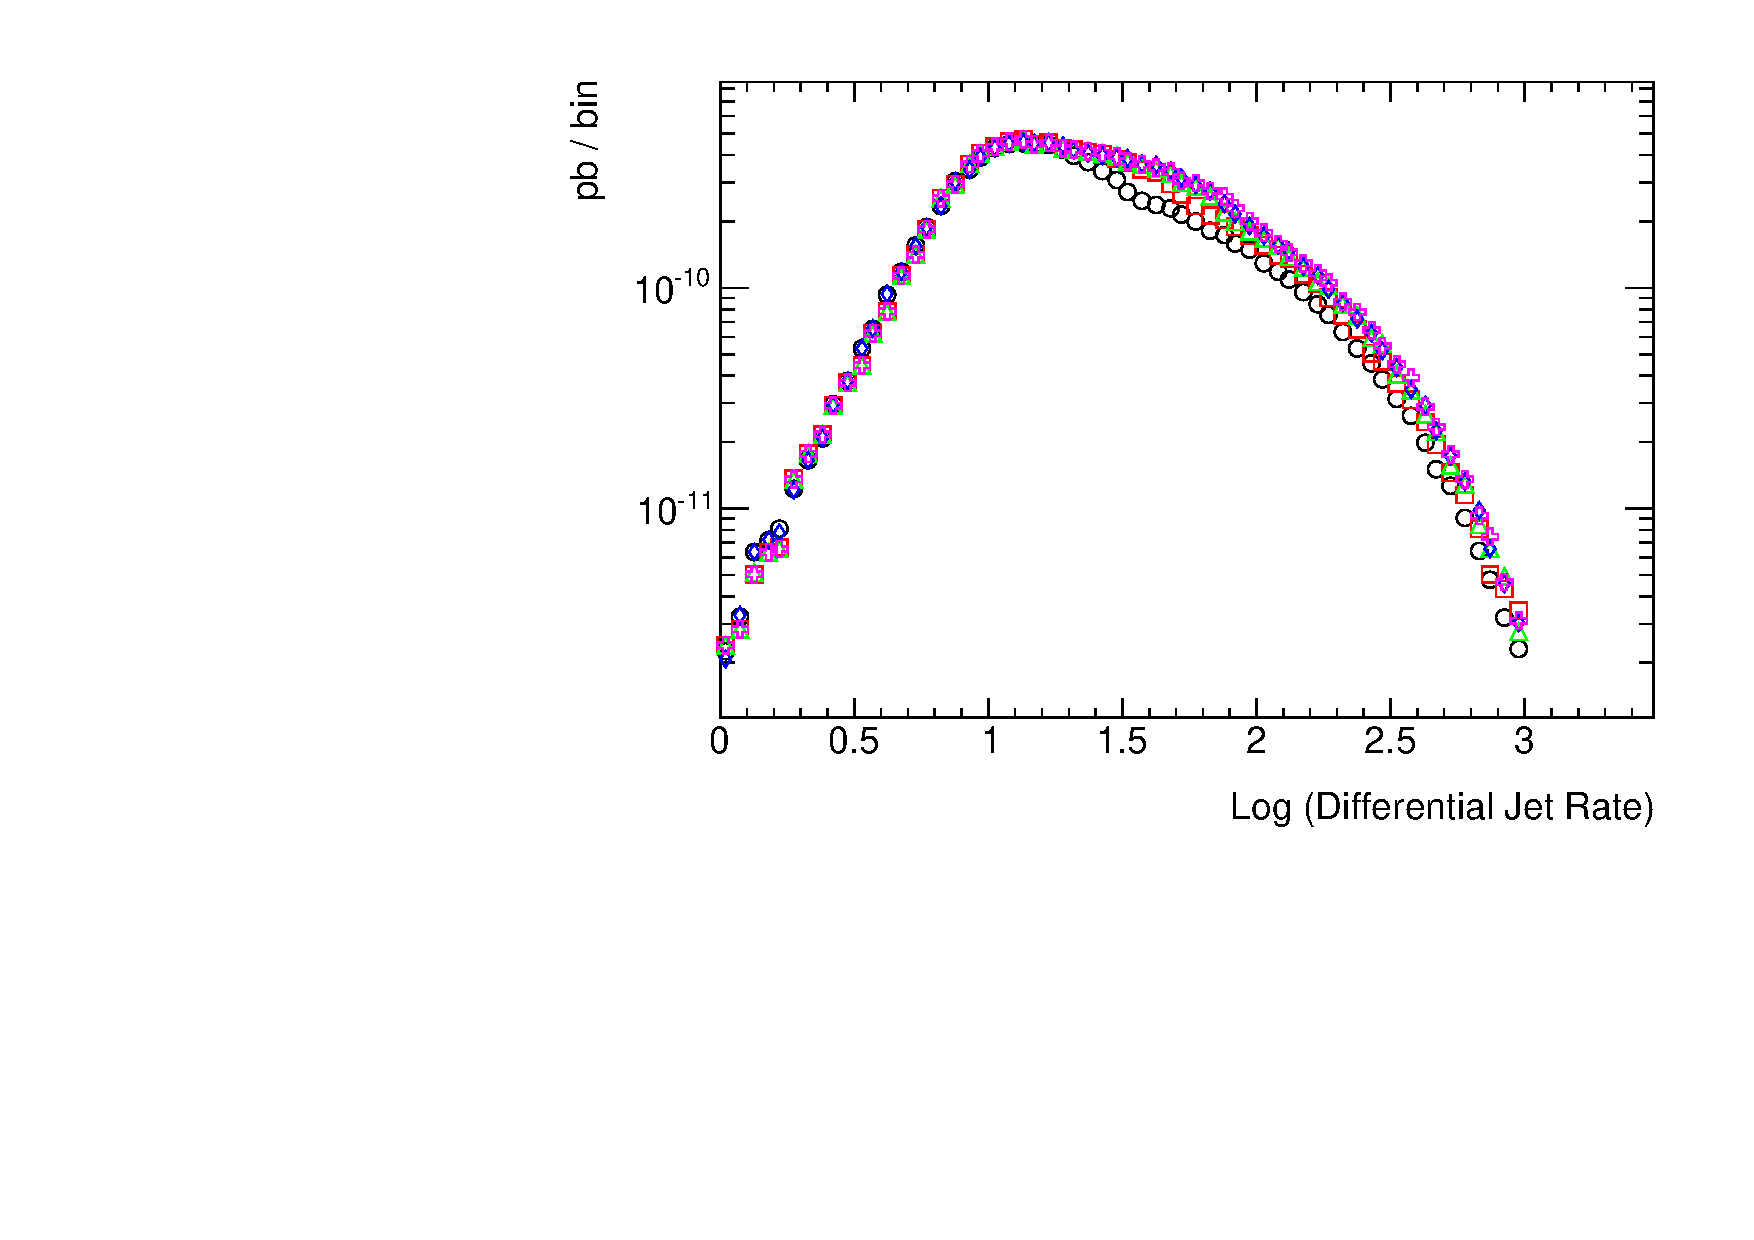
\includegraphics[width=0.48\linewidth]{figures/monojet_appendix/compare_plot_1.pdf}
		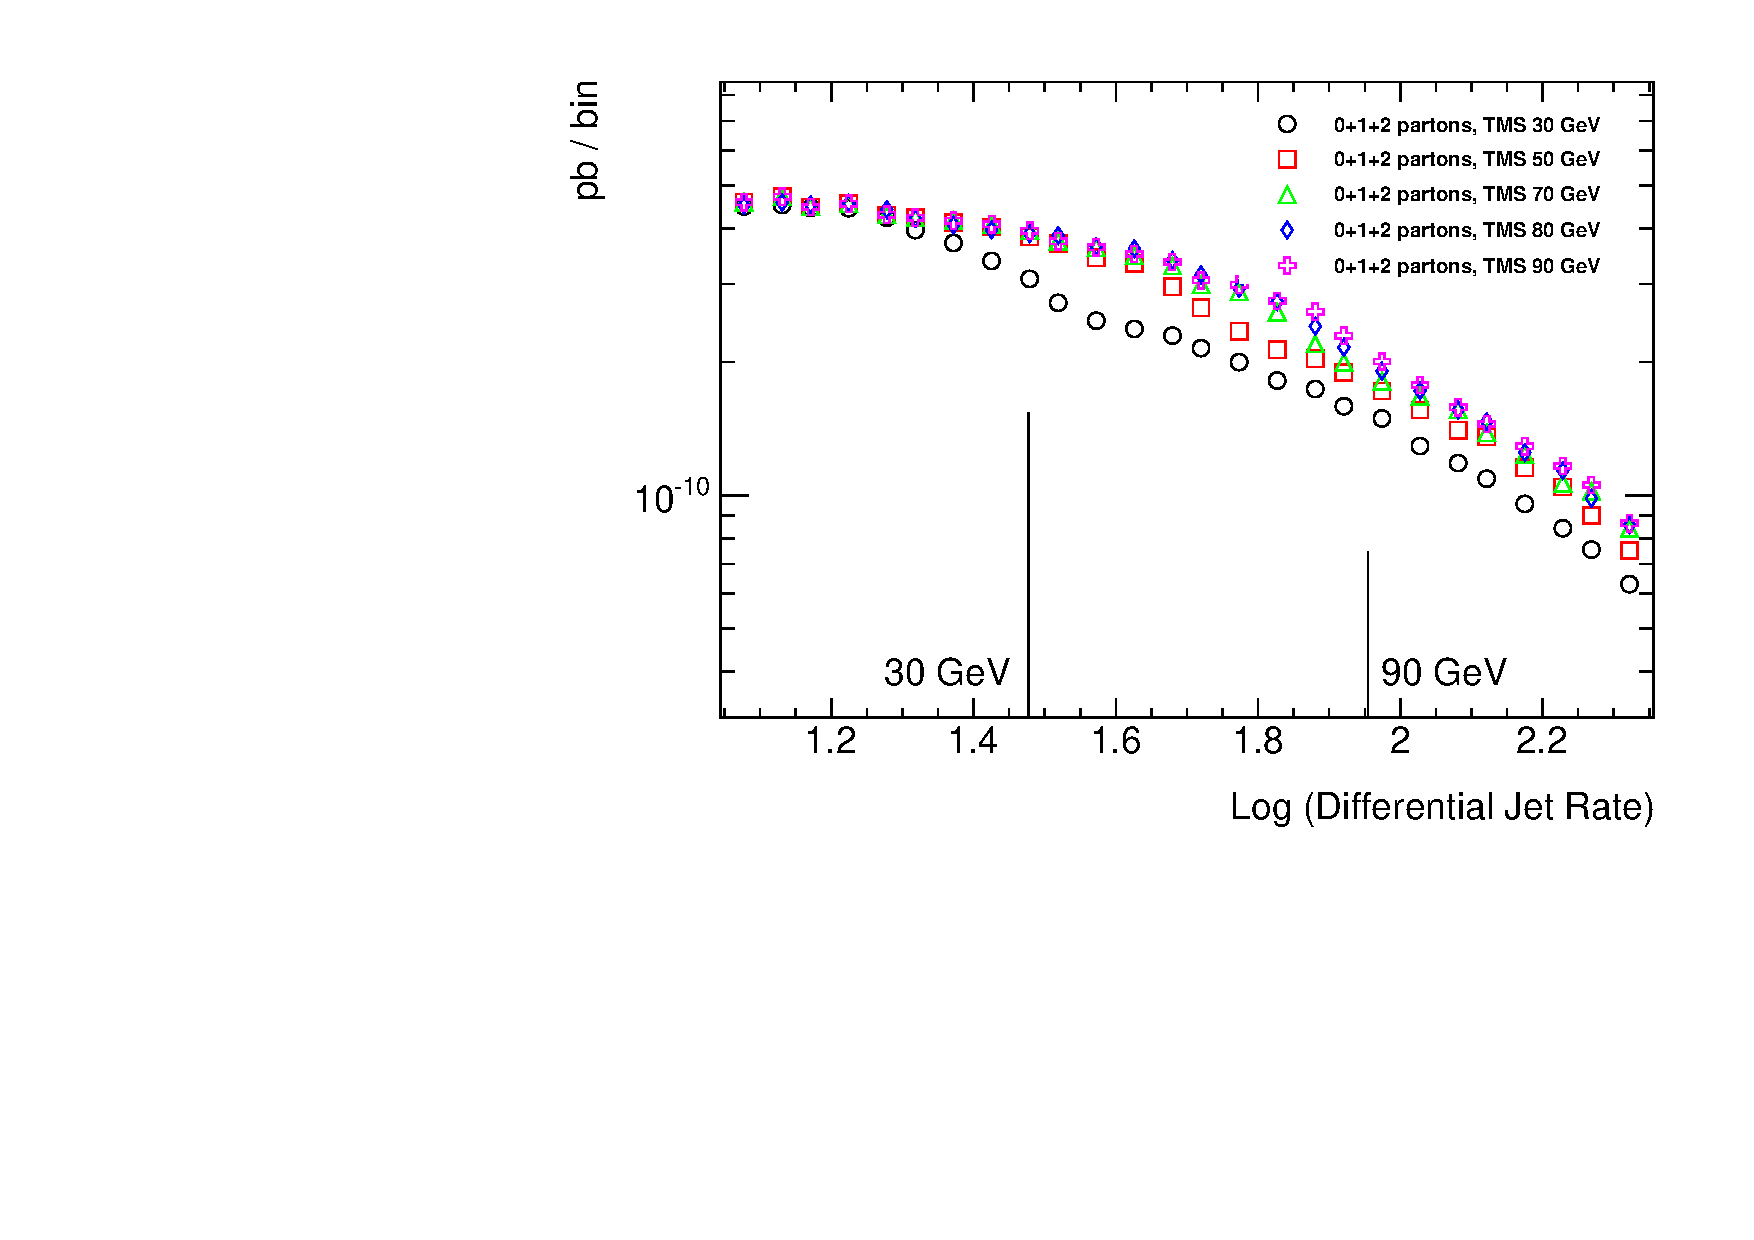
\includegraphics[width=0.48\linewidth]{figures/monojet_appendix/window_plot_1.pdf}
	}
	\hfill
	\subfloat[$2\rightarrow3$ parton process]{%
		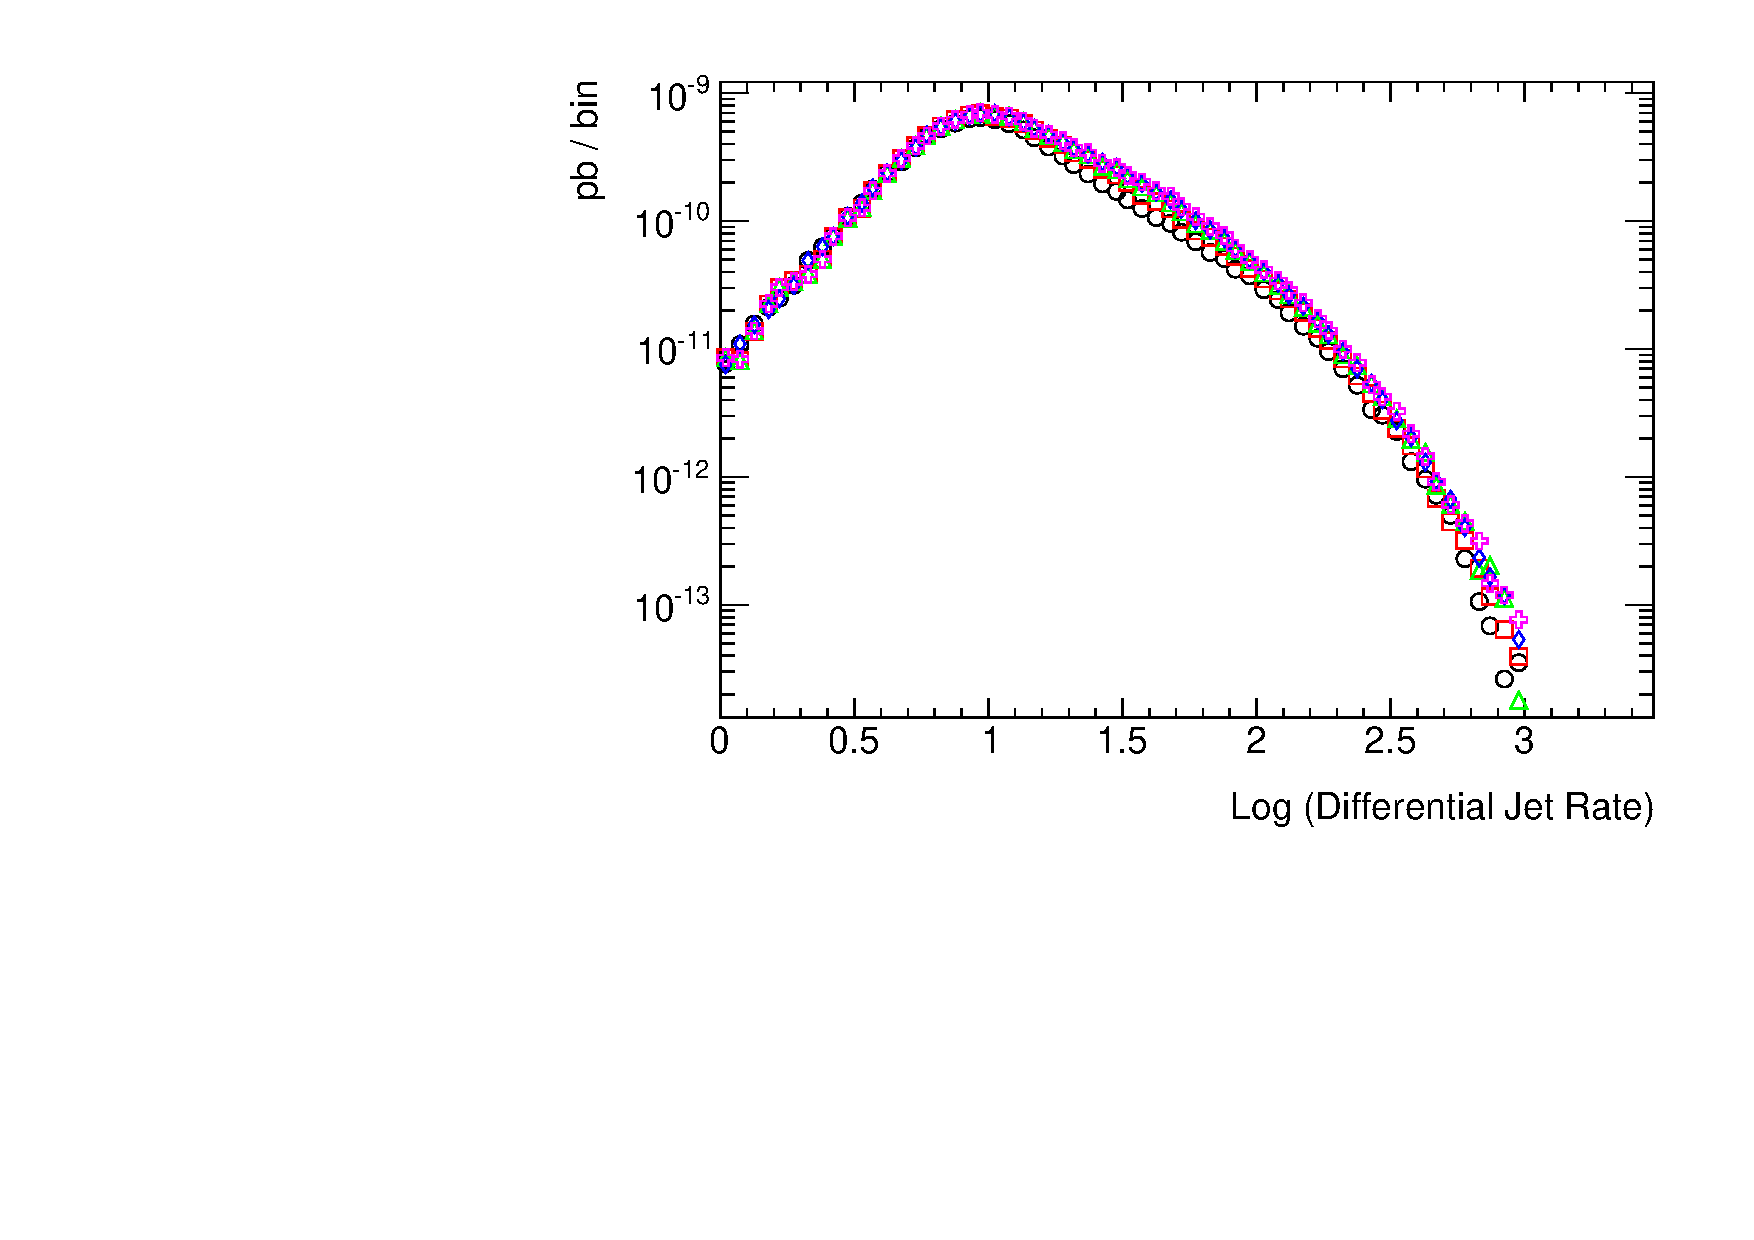
\includegraphics[width=0.48\linewidth]{figures/monojet_appendix/compare_plot_2.pdf}
		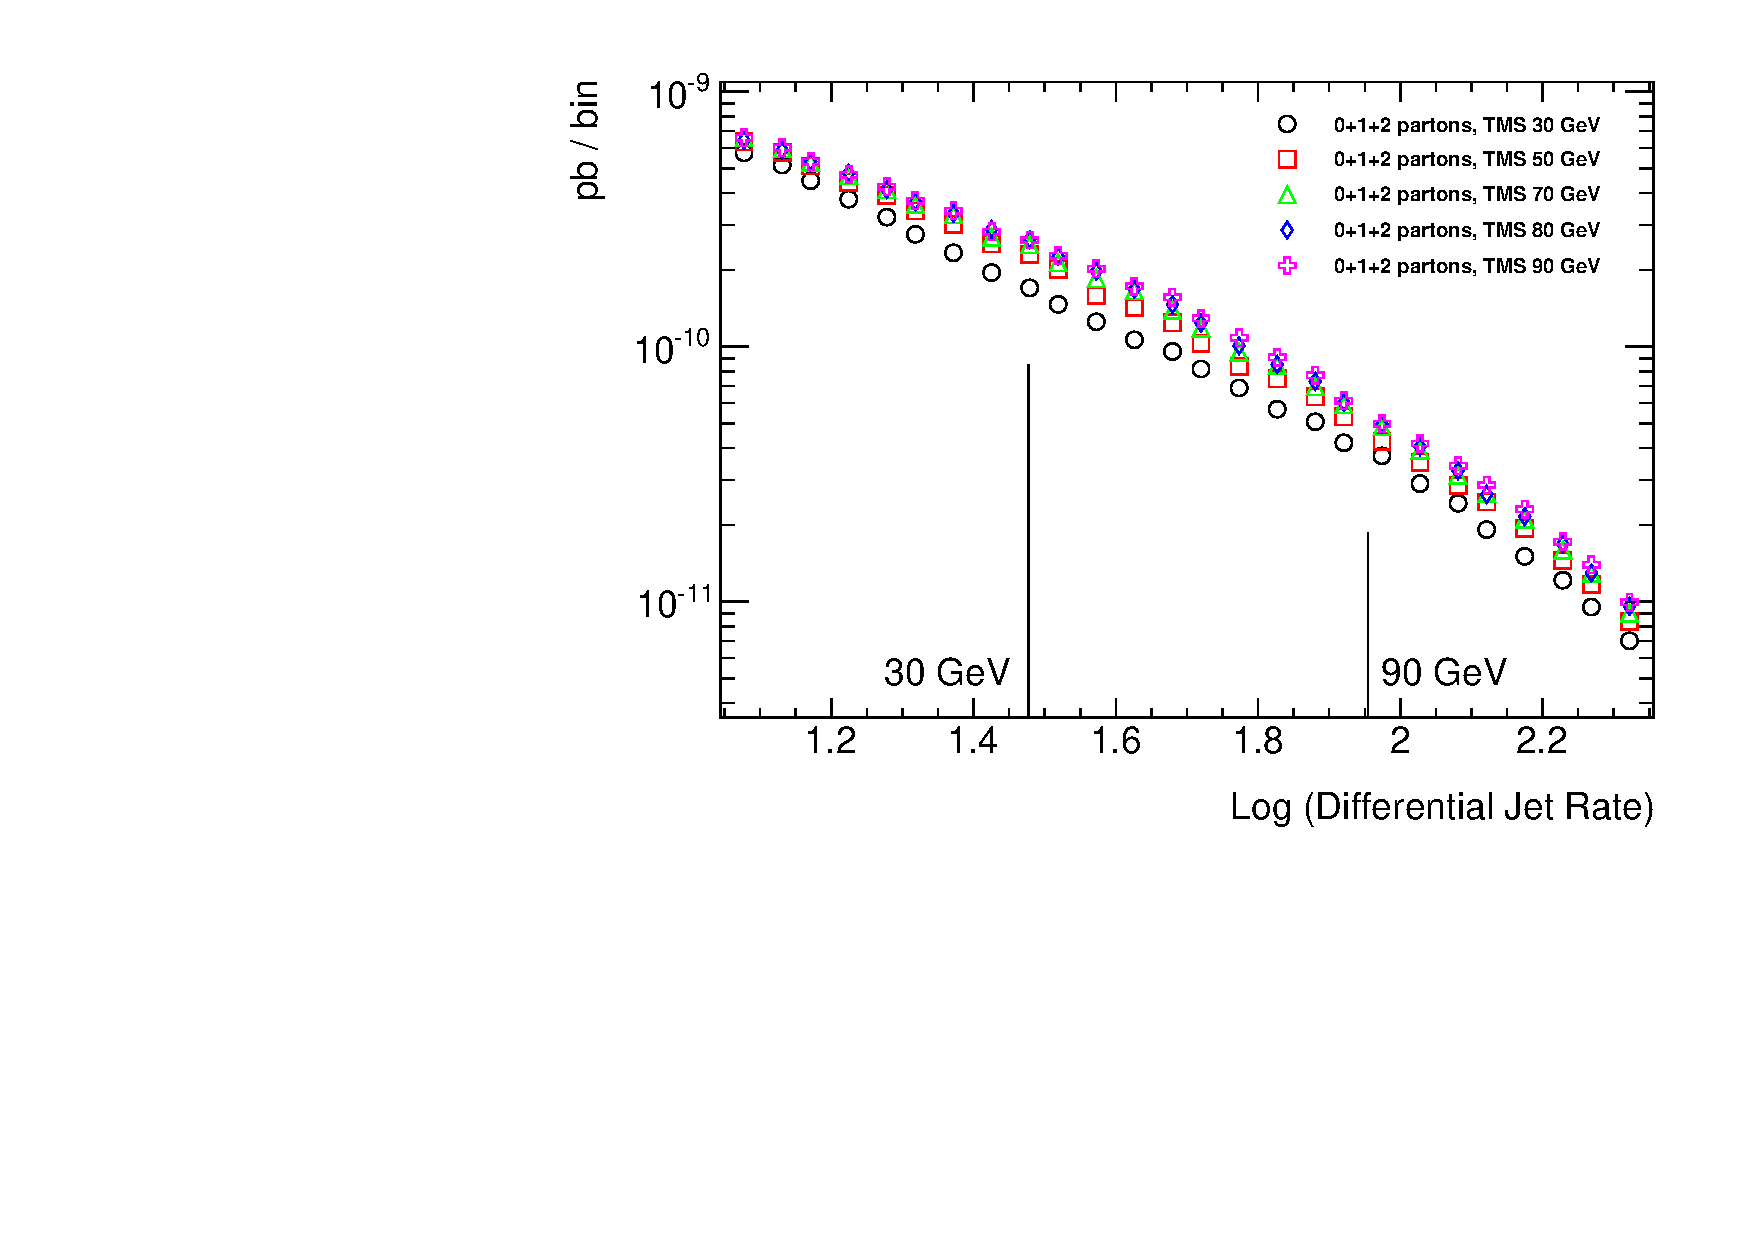
\includegraphics[width=0.48\linewidth]{figures/monojet_appendix/window_plot_2.pdf}
	}
	\hfill
	\subfloat[$3\rightarrow4$ parton process]{%
		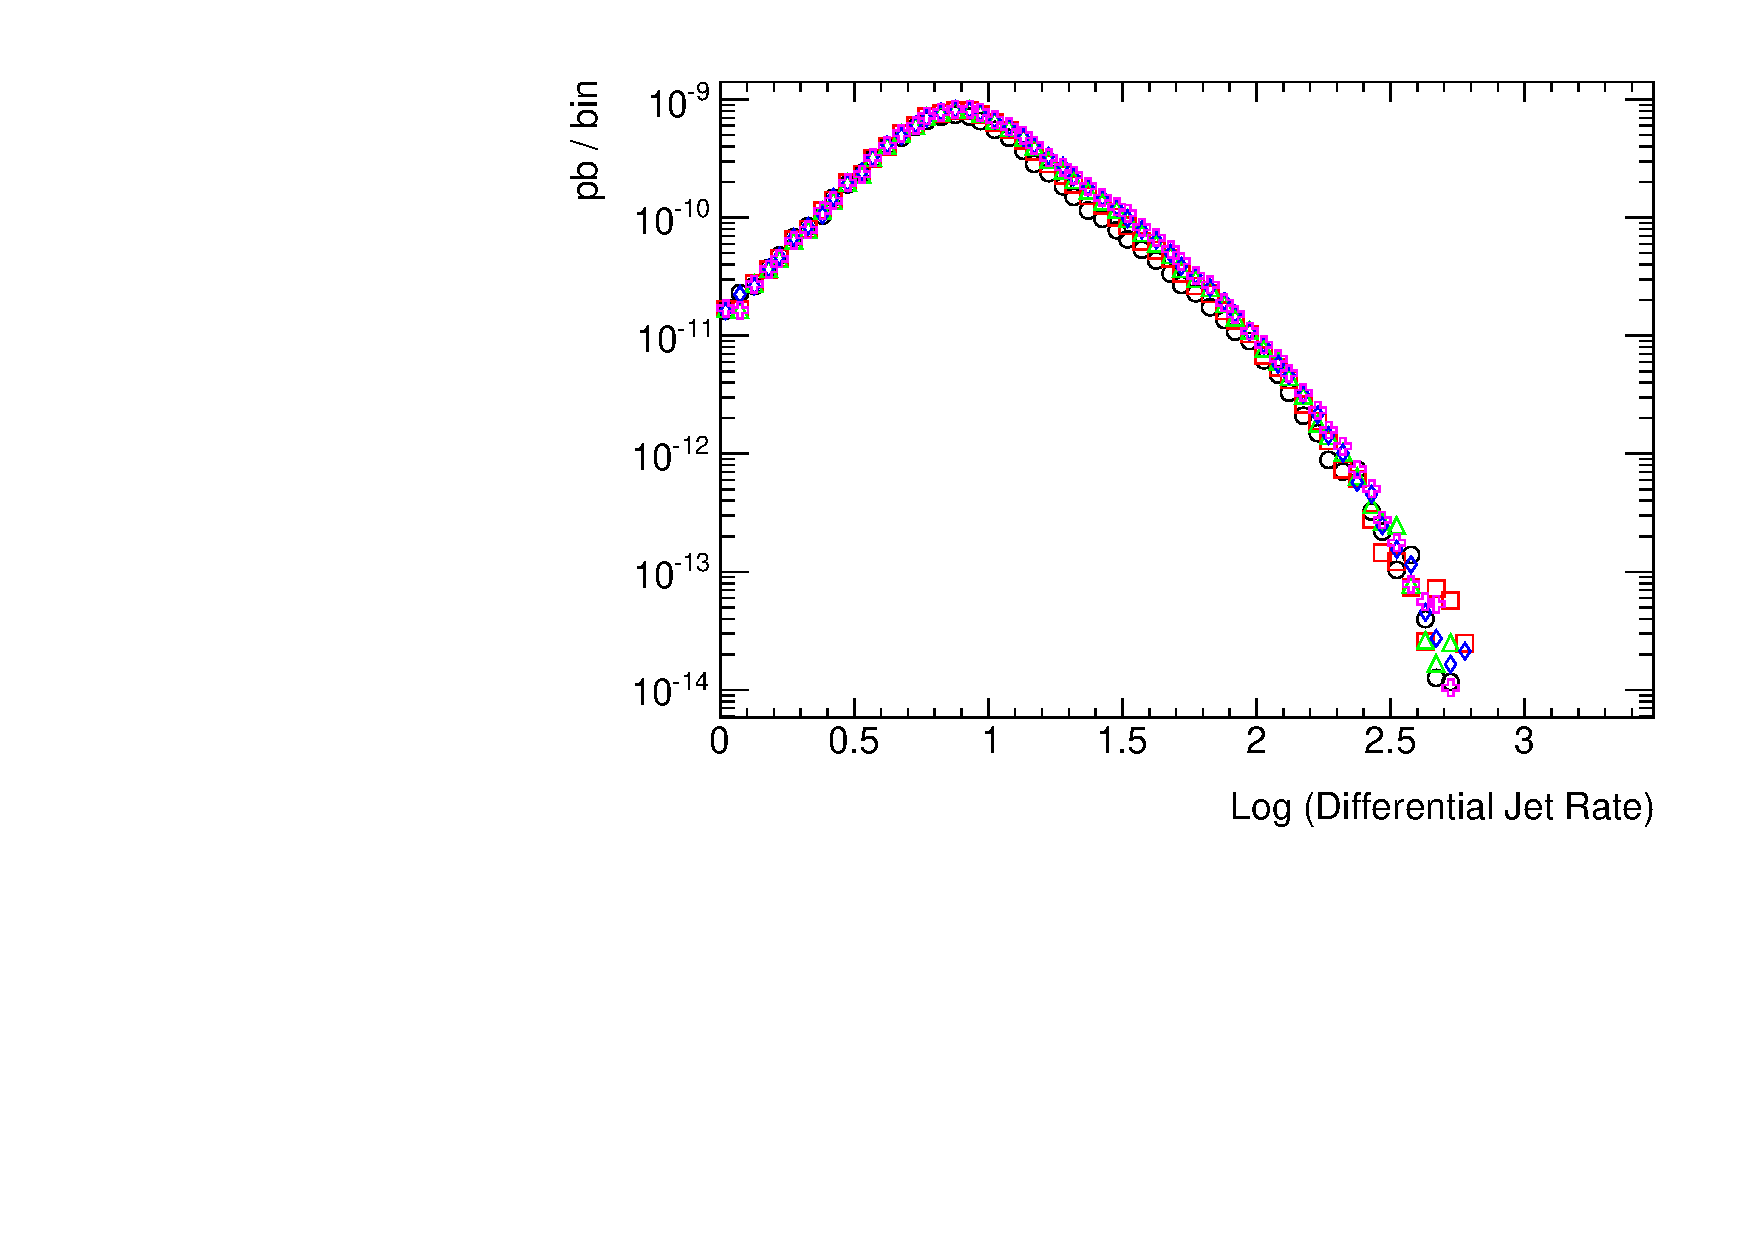
\includegraphics[width=0.48\linewidth]{figures/monojet_appendix/compare_plot_3.pdf}
		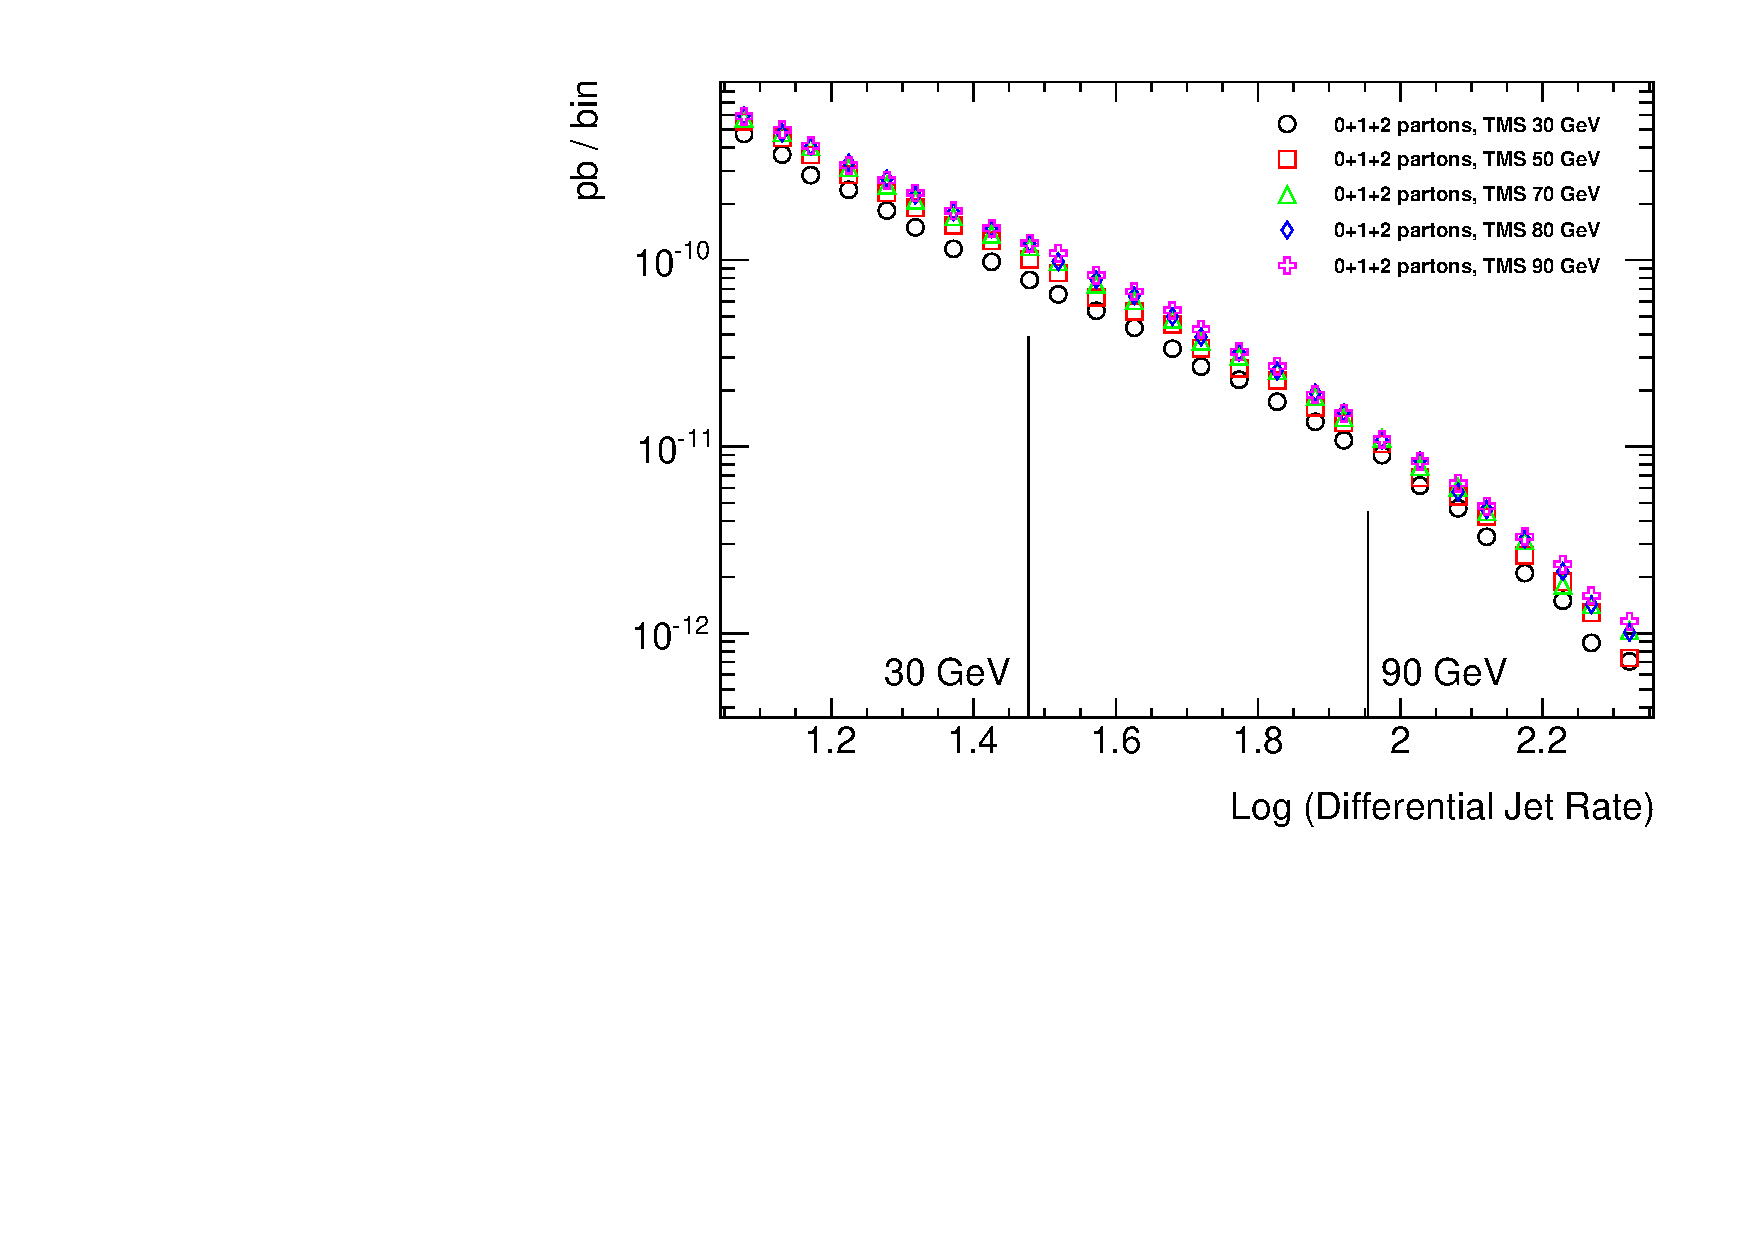
\includegraphics[width=0.48\linewidth]{figures/monojet_appendix/window_plot_3.pdf}
	}
	\hfill
	\subfloat[$4\rightarrow5$ parton process]{%
		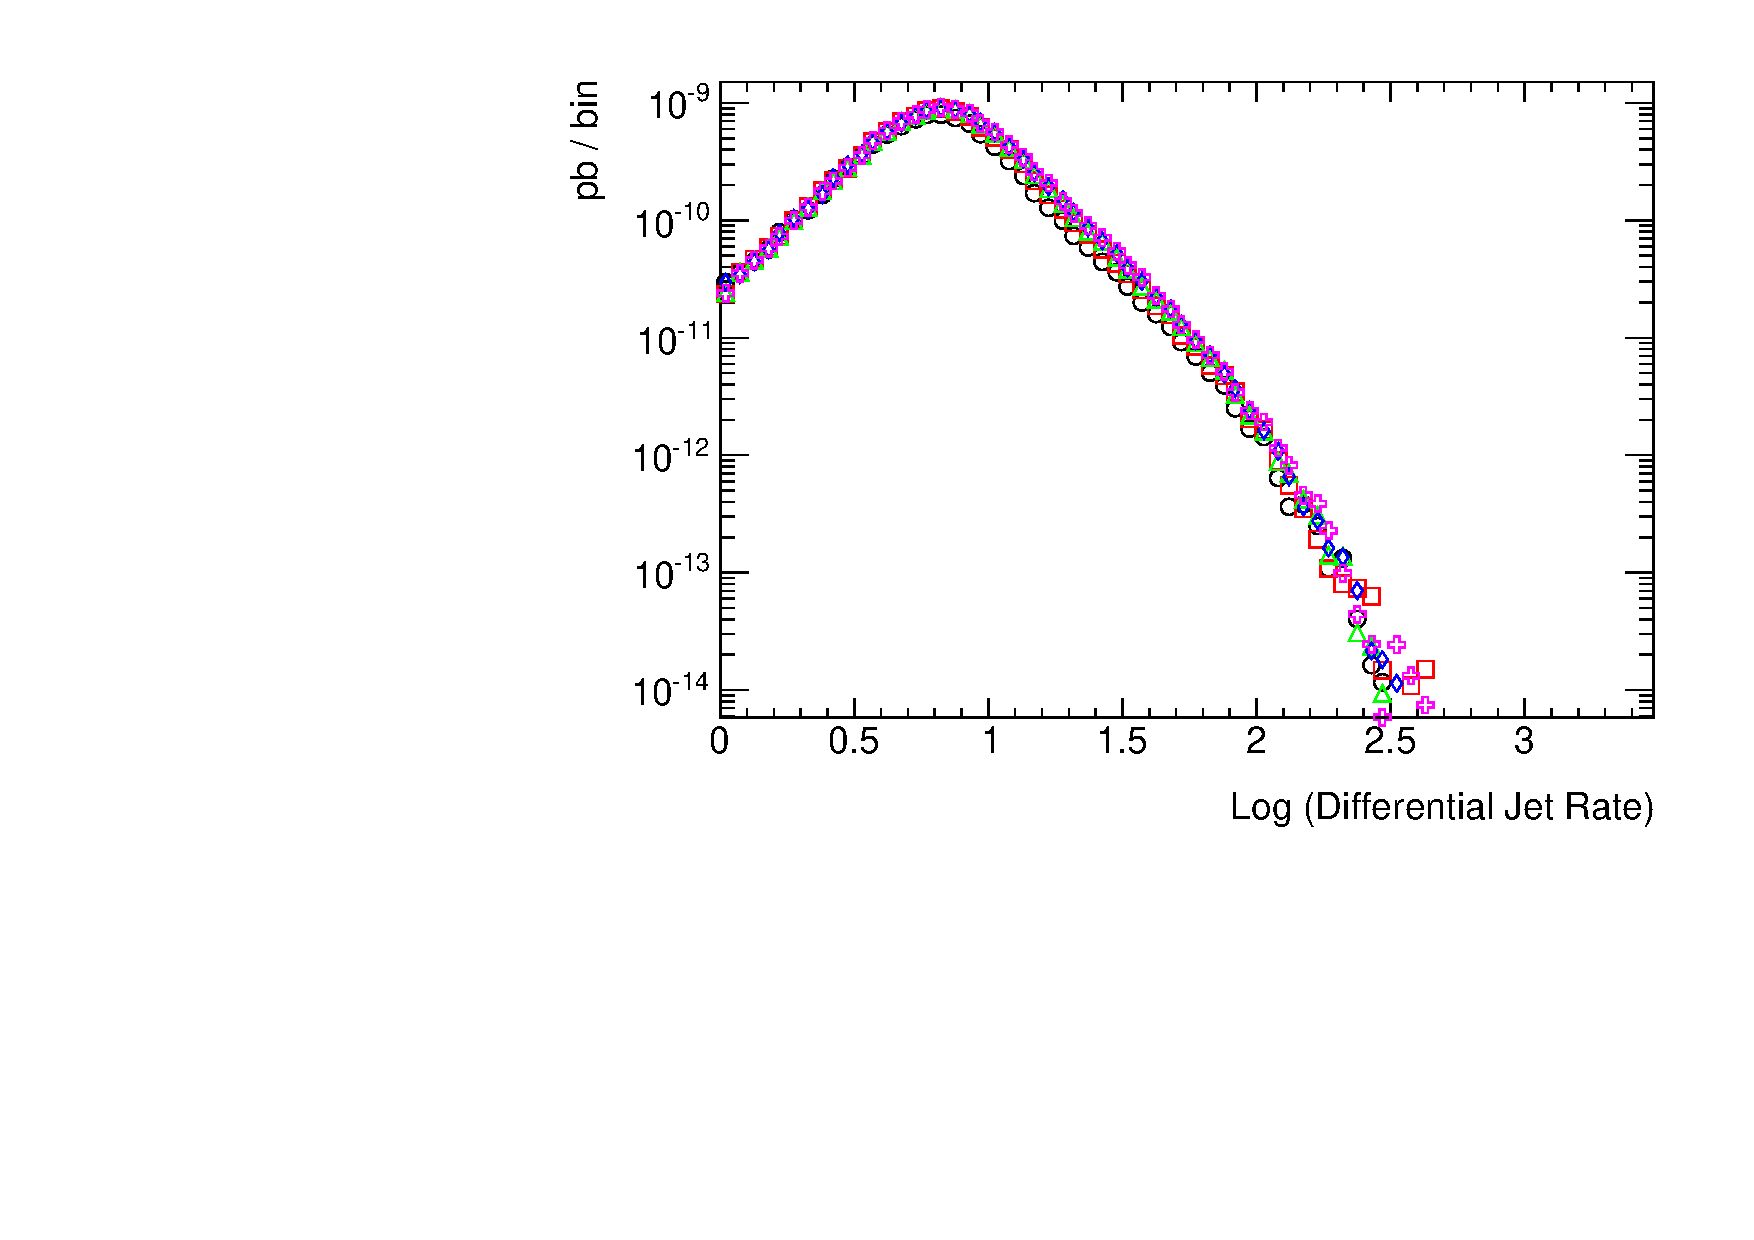
\includegraphics[width=0.48\linewidth]{figures/monojet_appendix/compare_plot_4.pdf}
		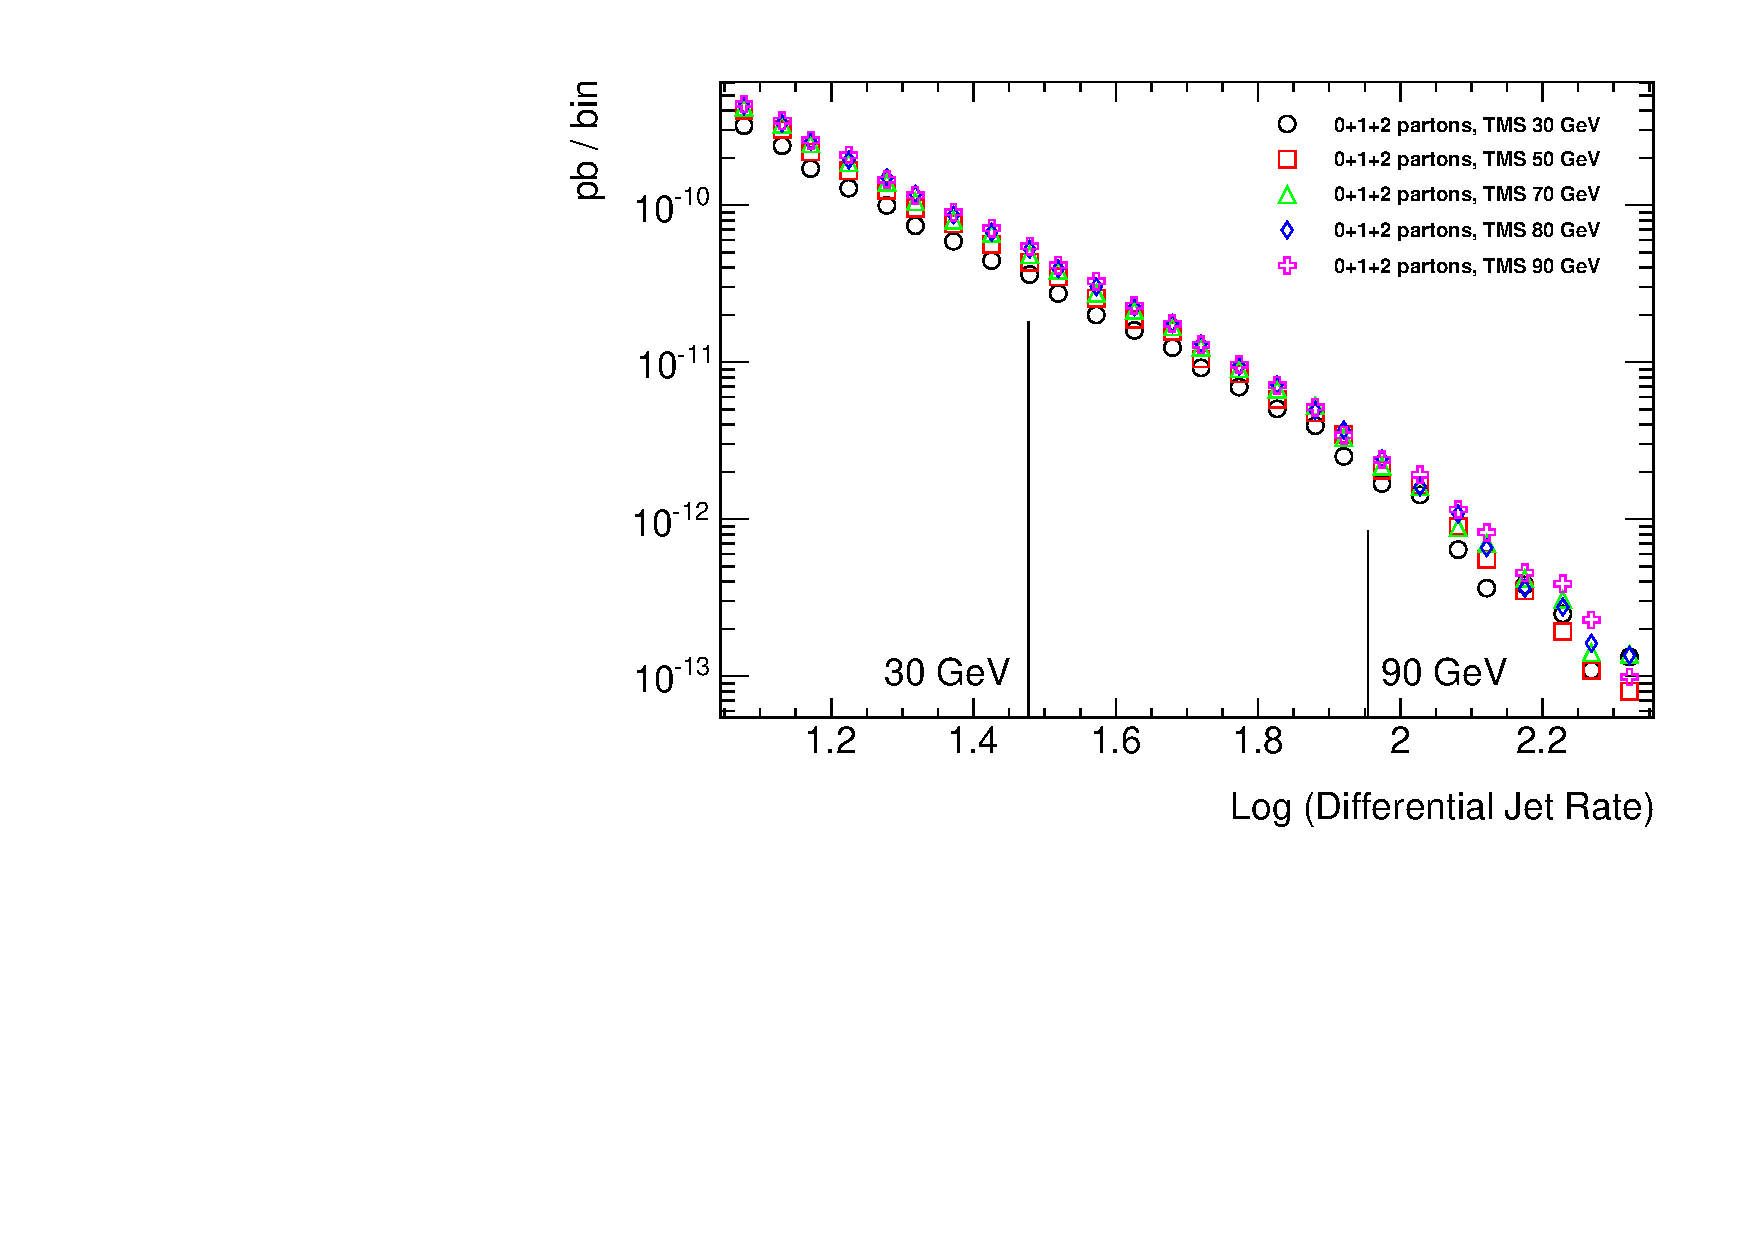
\includegraphics[width=0.48\linewidth]{figures/monojet_appendix/window_plot_4.pdf}
	}
  \caption{Jet differential rates distributions for EFT D5 sample with CKKW matching scale at 30, 50, 70, 80 and 90 GeV. 0-, 1- and 2-parton emission cases are generated separatedly and the total merged contribution is shown. A closer look is shown around the matching scale.}
  \label{fig:CKKW_D5_zoom}
\end{figure}


The MC distributions for the missing transverse energy and transverse momenta for the leading and subleading jets are plotted in Fig.. For the mono-jet analysis, usually a missing transverse energy cut larger than 300 GeV is applied for offline selection, which makes the contribution of the 0-parton emission case negligible in the mono-jet analysis.

\begin{figure}[h!]
	\centering  
%	\subfloat[Missing transverse momentum]{%
    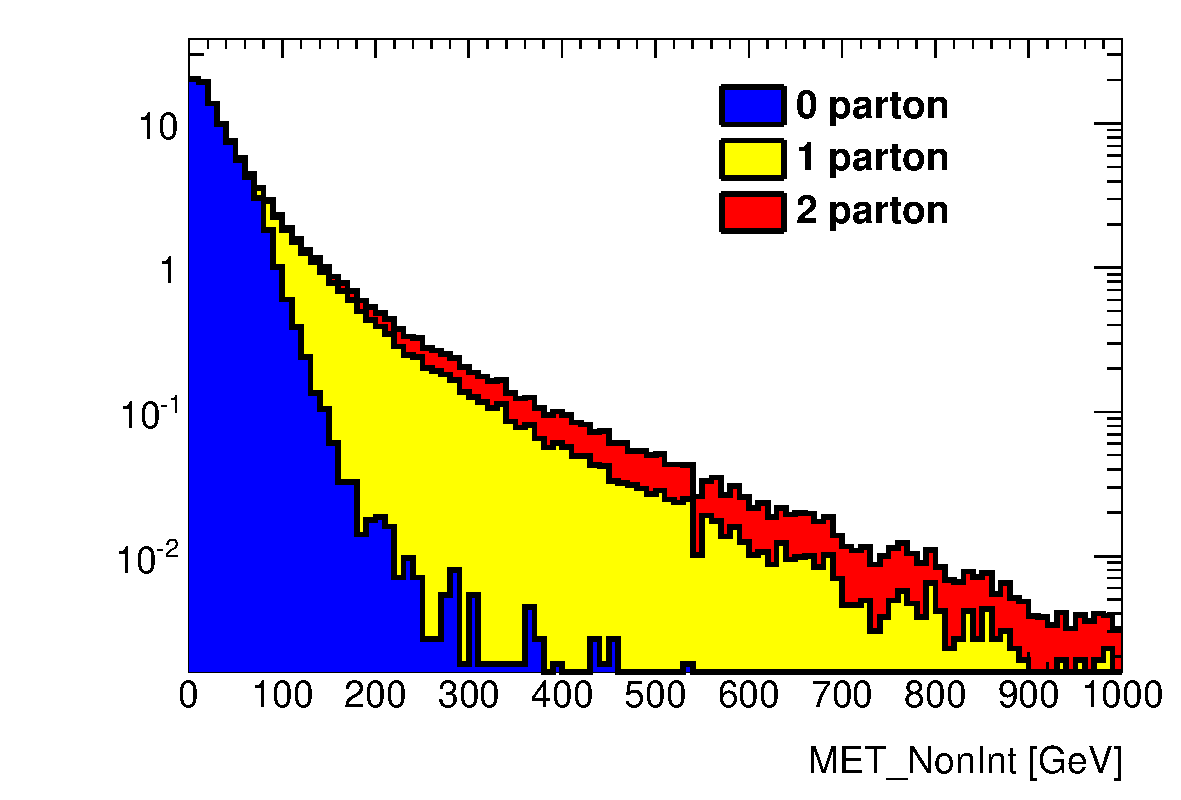
\includegraphics[width=0.8\linewidth]{figures/monojet_appendix/MET_matching80.pdf}
%	}
%	\hfill
%	\subfloat[Transverse momentum of leading jet]{%
%    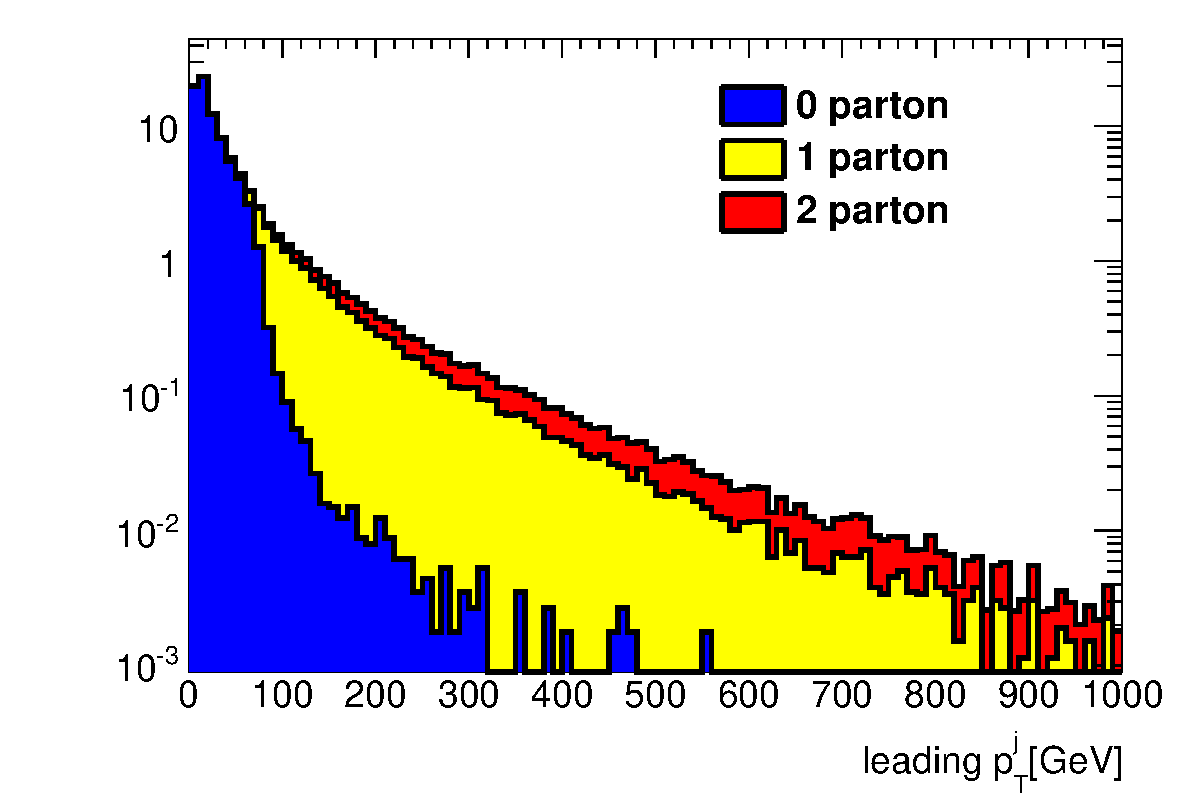
\includegraphics[width=0.48\linewidth]{figures/monojet_appendix/jet1pt_matching80.pdf}
%	}
%	\hfill
%	\subfloat[Transverse momentum of subleading jet]{%
%    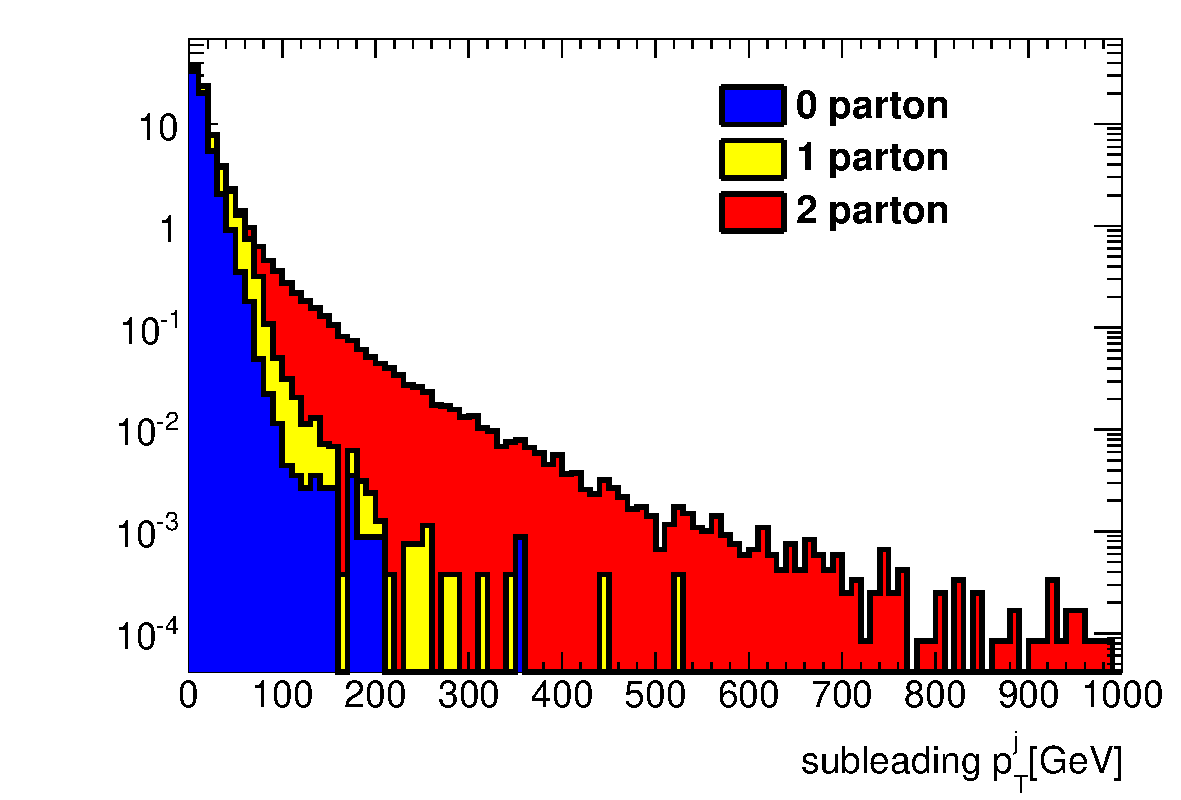
\includegraphics[width=0.48\linewidth]{figures/monojet_appendix/jet2pt_matching80.pdf}
%	}
%	\caption{Kinematics distributions for EFT D5 sample with CKKW matching scale at 80 GeV. 0-, 1- and 2-parton emission cases are generated separatedly and added together by cross sections. The 0-parton emission case has very limited contribution for missing transverse energy larger than 300 GeV region.}
	\caption{Missing transverse momentum distributions for EFT D5 sample with CKKW matching scale at 80 GeV. 0-, 1- and 2-parton emission cases are generated separatedly and added together by cross sections. The 0-parton emission case has very limited contribution for missing transverse energy larger than 300 GeV region.}
	\label{fig:Kine_D5_80}
\end{figure}


\section{Parton emission generation}
\label{sec:monojet_parton_emission}
In order to describe the signal kinematics correctly and save time in MC generation, the parton emissions will only be generated up to a certain numbers of parton and ignore the cases with more partons. The later ones usually have cross sections small enough and limited contribution in the interested kinematic regions.

It is found that the 3- or more-parton emission cases are negligible in our intersted regions, but the 2-parton emission case has significant contributions. The 0- and 1-parton emissions are out of discussion since they give the baseline signature in this analysis. The impacts of 2- and 3-parton emissions are quantified in this section.

Here the 0-, 1-, 2- and 3-parton emissions are generated separately and requested in matching step with \texttt{Merging:nJetMax=3} and scale at 80 GeV in Pythia8for 0+1+2+3 parton emission case, while \texttt{Merging:nJetMax=2} requested for 0+1+2 case and \texttt{Merging:nJetMax=1} requested for 0+1 case. The MET distribution is plotted in Fig.\ref{fig:RatioKine_D5}, while the jet multiplicity is shown in Fig.\ref{fig:RatioKine_D5_2}.

\begin{figure}[h!]
	\centering  
%	\subfloat[Missing transverse momentum]{%
	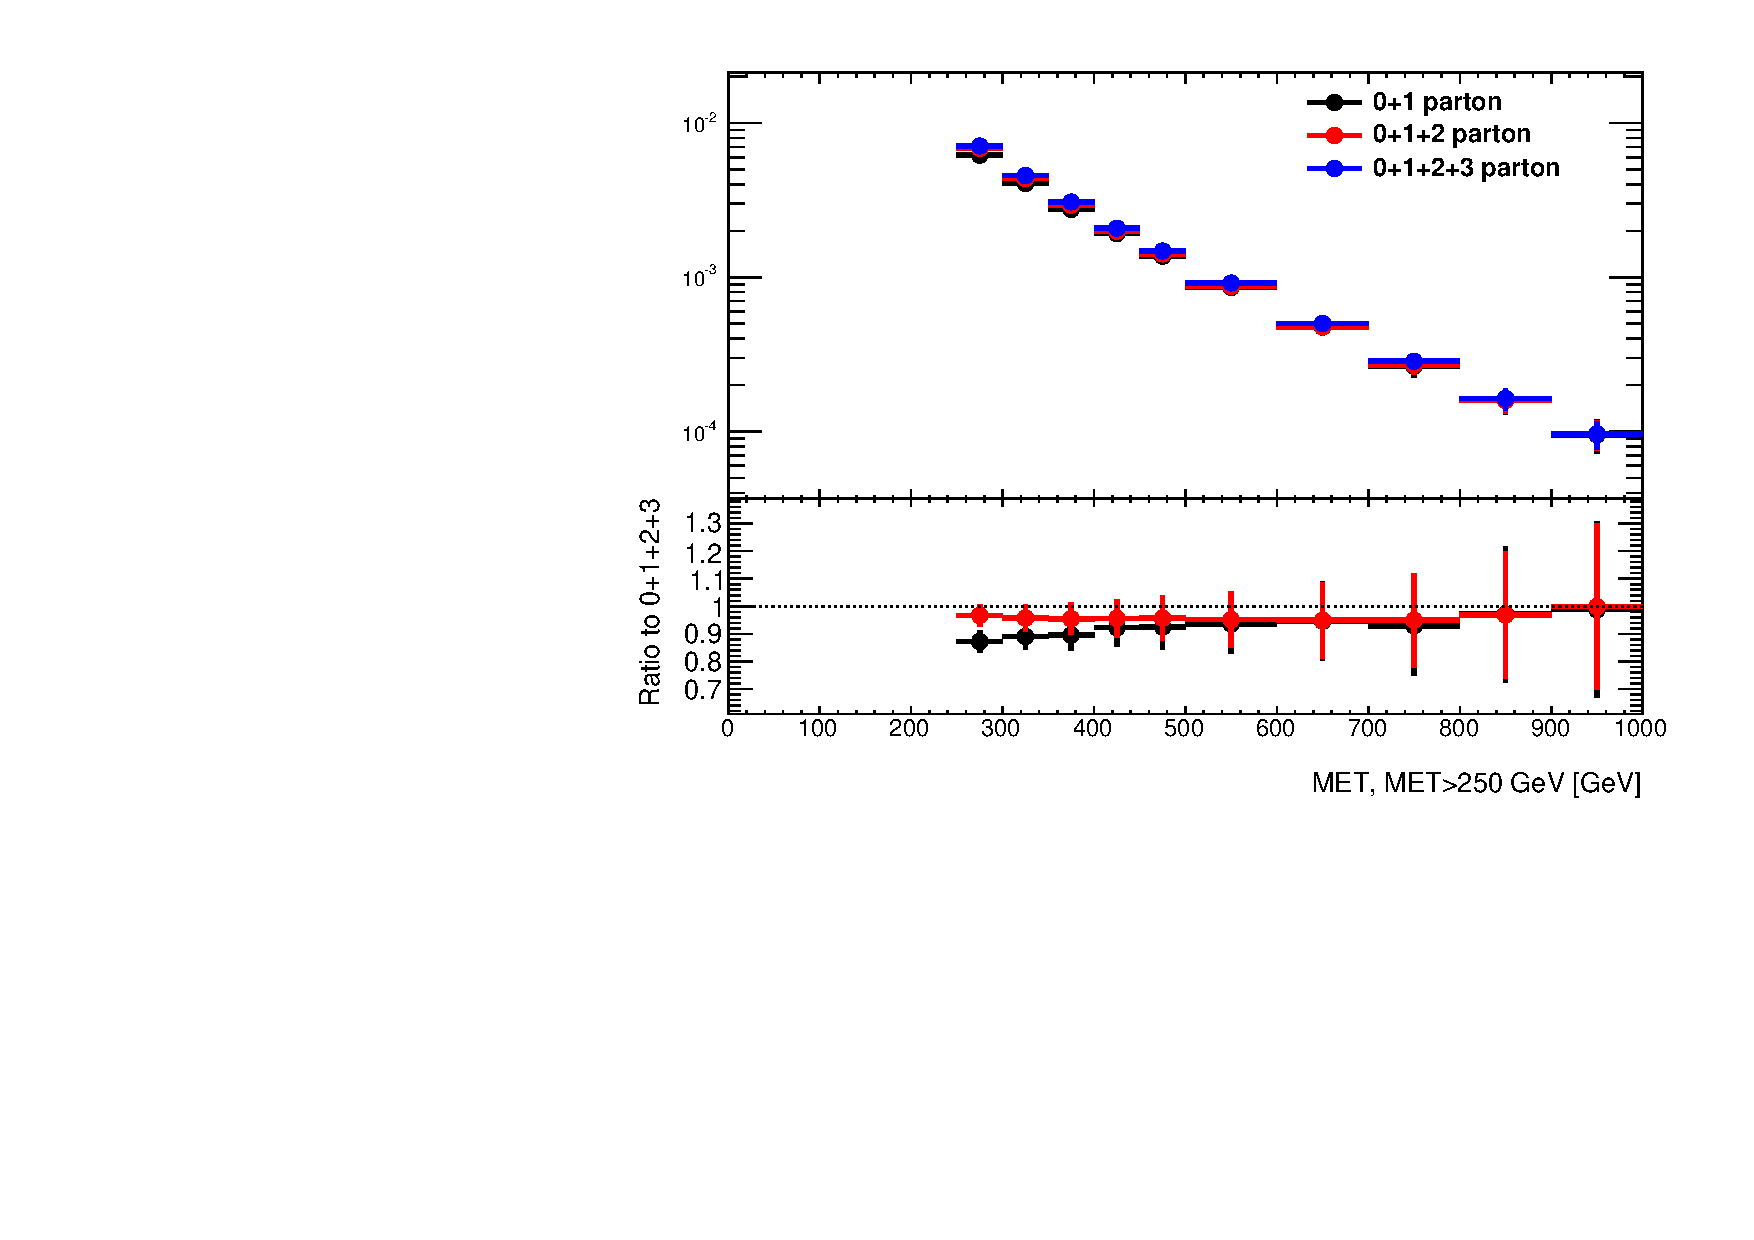
\includegraphics[width=0.8\linewidth]{figures/monojet_appendix/h_MET_MET250.pdf}
%	}
%	\hfill
%	\subfloat[Transverse momentum of leading jet]{%
%		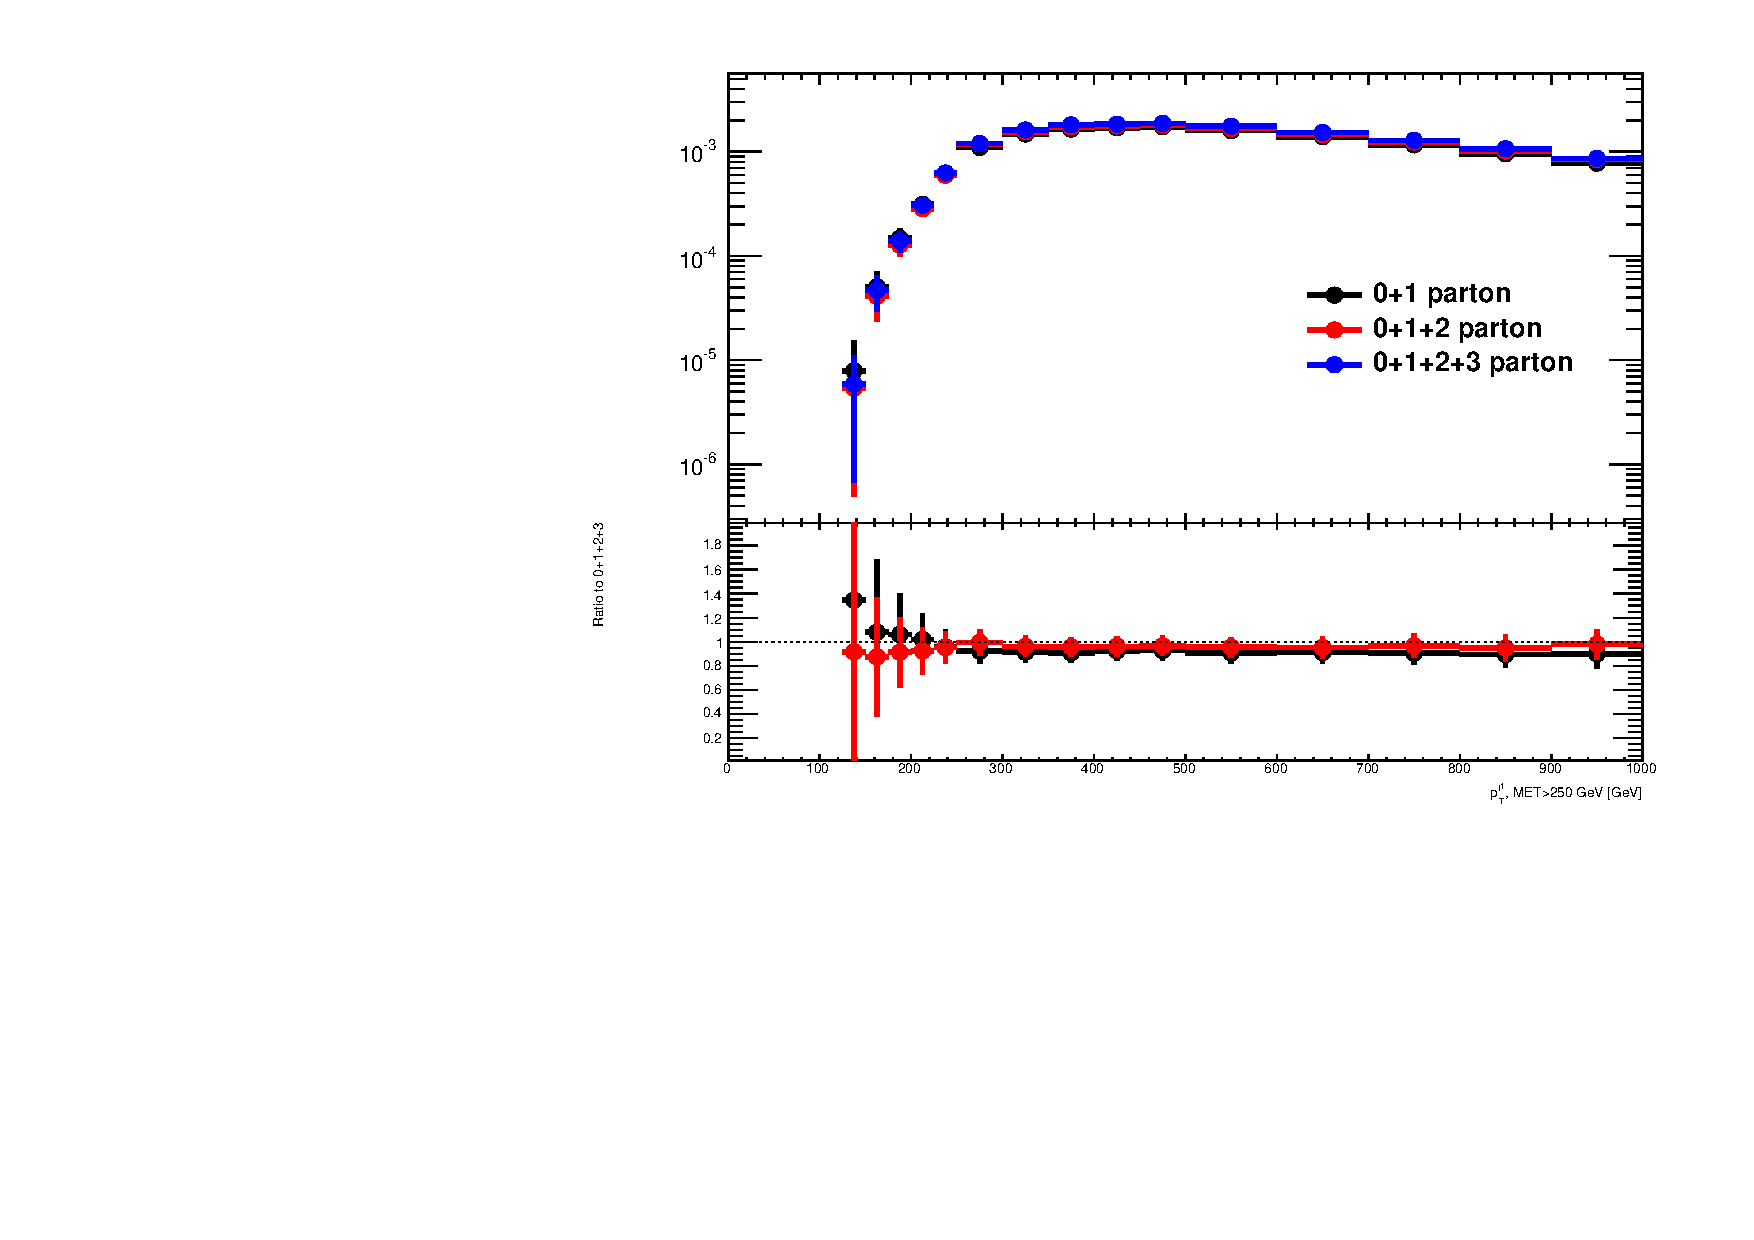
\includegraphics[width=0.48\linewidth]{figures/monojet_appendix/h_pt1_MET250.pdf}
%	}
%	\hfill
%	\subfloat[Transverse momentum of subleading jet]{%
%		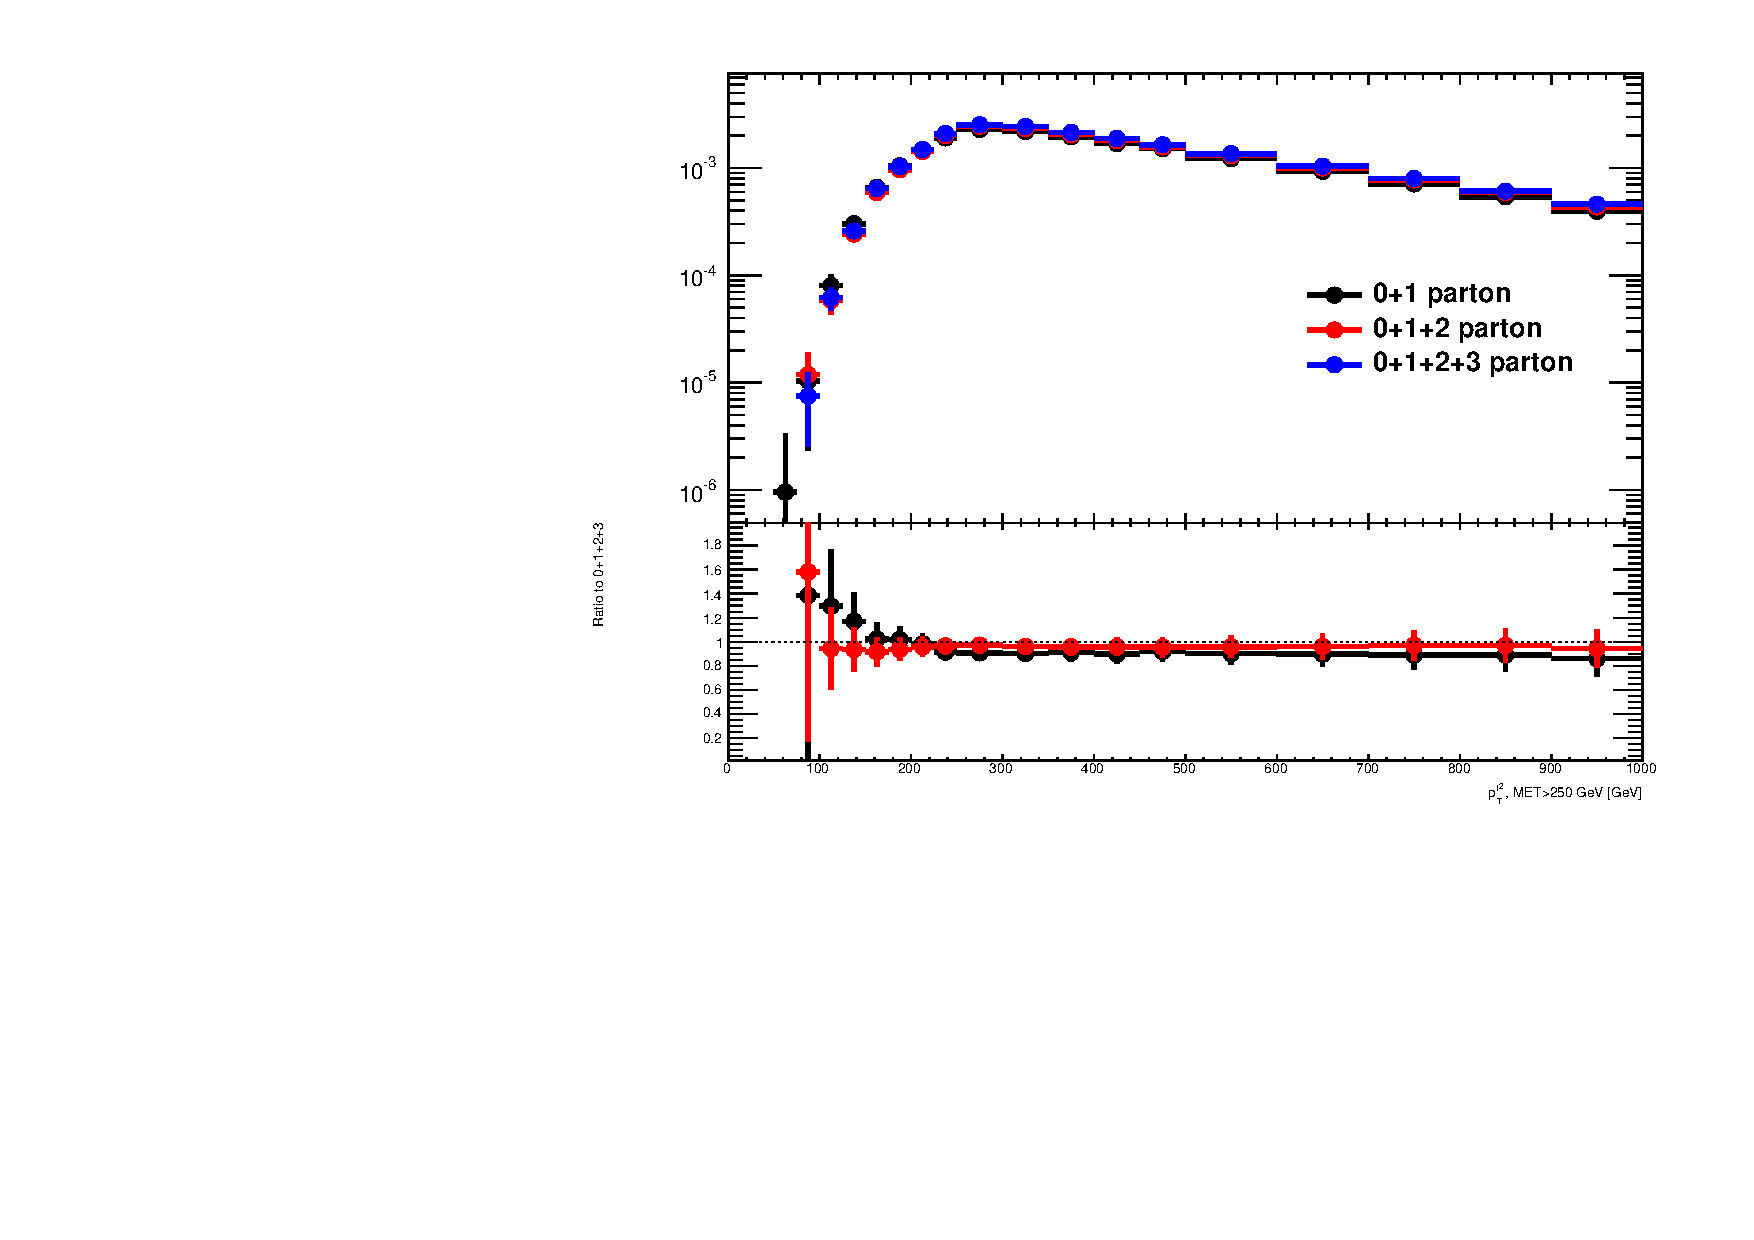
\includegraphics[width=0.48\linewidth]{figures/monojet_appendix/h_pt2_MET250.pdf}
%	}
%	\caption{Kinematics distributions for EFT D5 sample with CKKW matching scale at 80 GeV. 0-, 1-, 2- and 3-parton emission cases are generated separatedly and added together by cross sections.}
	\caption{Missing transverse momentum distributions for EFT D5 sample with CKKW matching scale at 80 GeV. 0-, 1-, 2- and 3-parton emission cases are generated separatedly and added together by cross sections.}
	\label{fig:RatioKine_D5}
\end{figure}


\begin{figure}[h!]
	\centering  
%	\subfloat[Jet multiplicity, leading jet $p_{T}>30$ GeV]{%
%    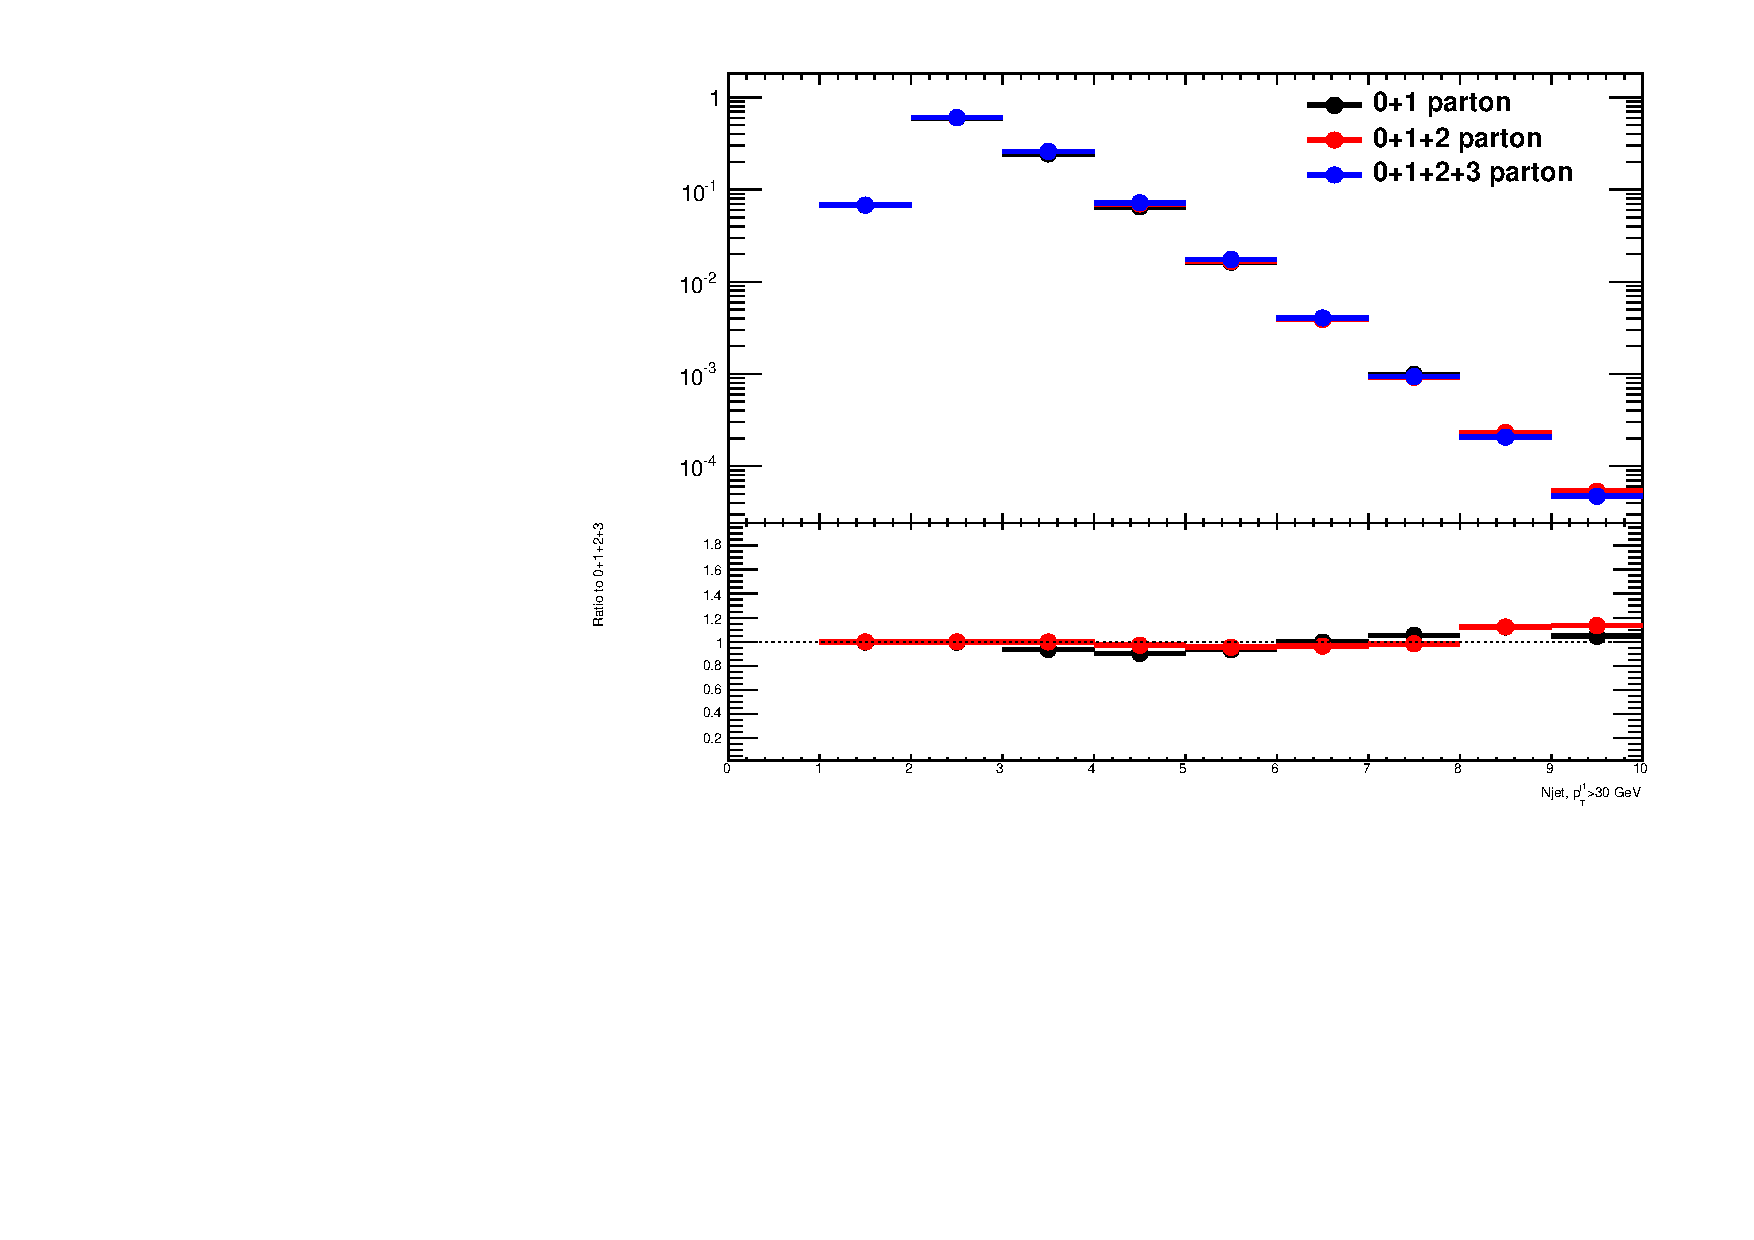
\includegraphics[width=0.48\linewidth]{figures/monojet_appendix/h_njet30.pdf}
%	}
%	\hfill
%	\subfloat[Jet multiplicity, leading jet $p_{T}>80$ GeV]{%
%    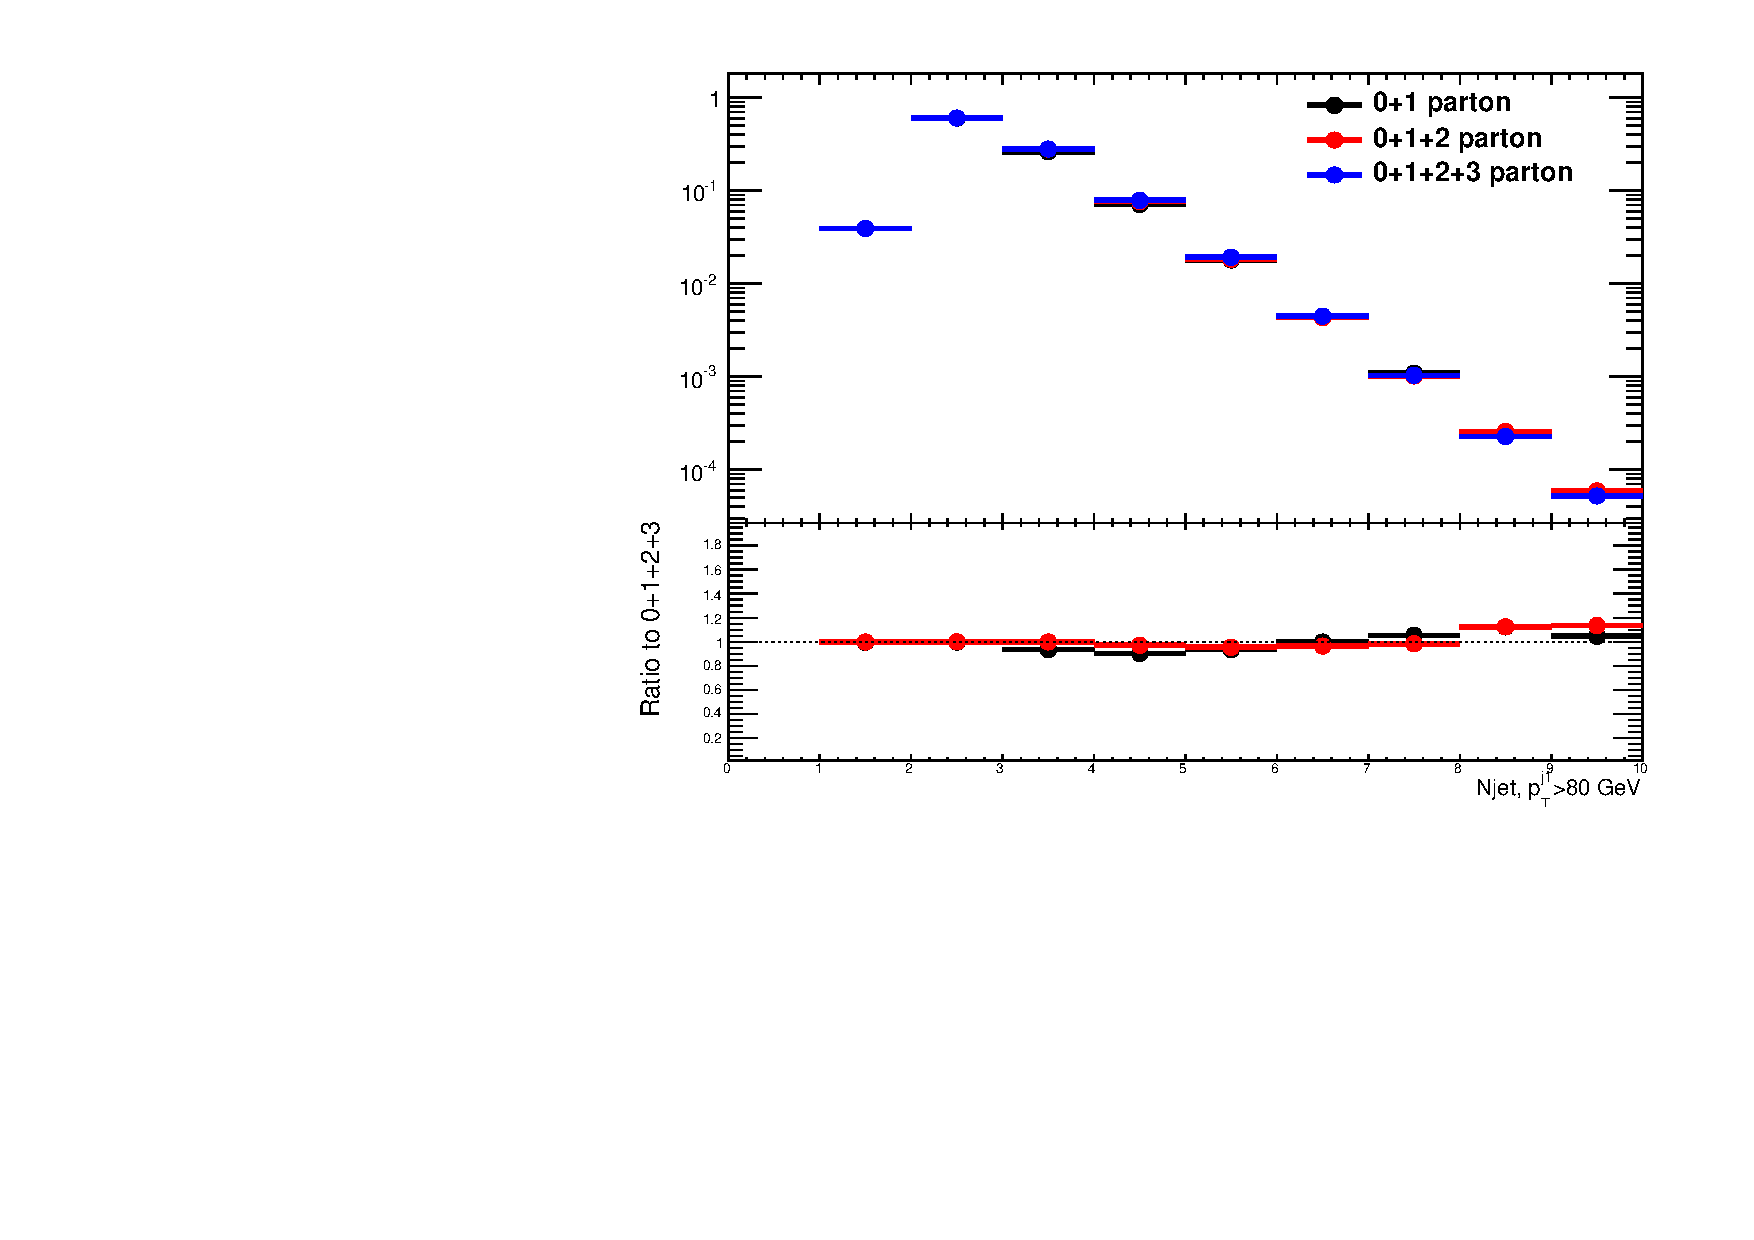
\includegraphics[width=0.48\linewidth]{figures/monojet_appendix/h_njet80.pdf}
%	}
%	\hfill
%	\subfloat[Jet multiplicity, leading jet $p_{T}>250$ GeV]{%
	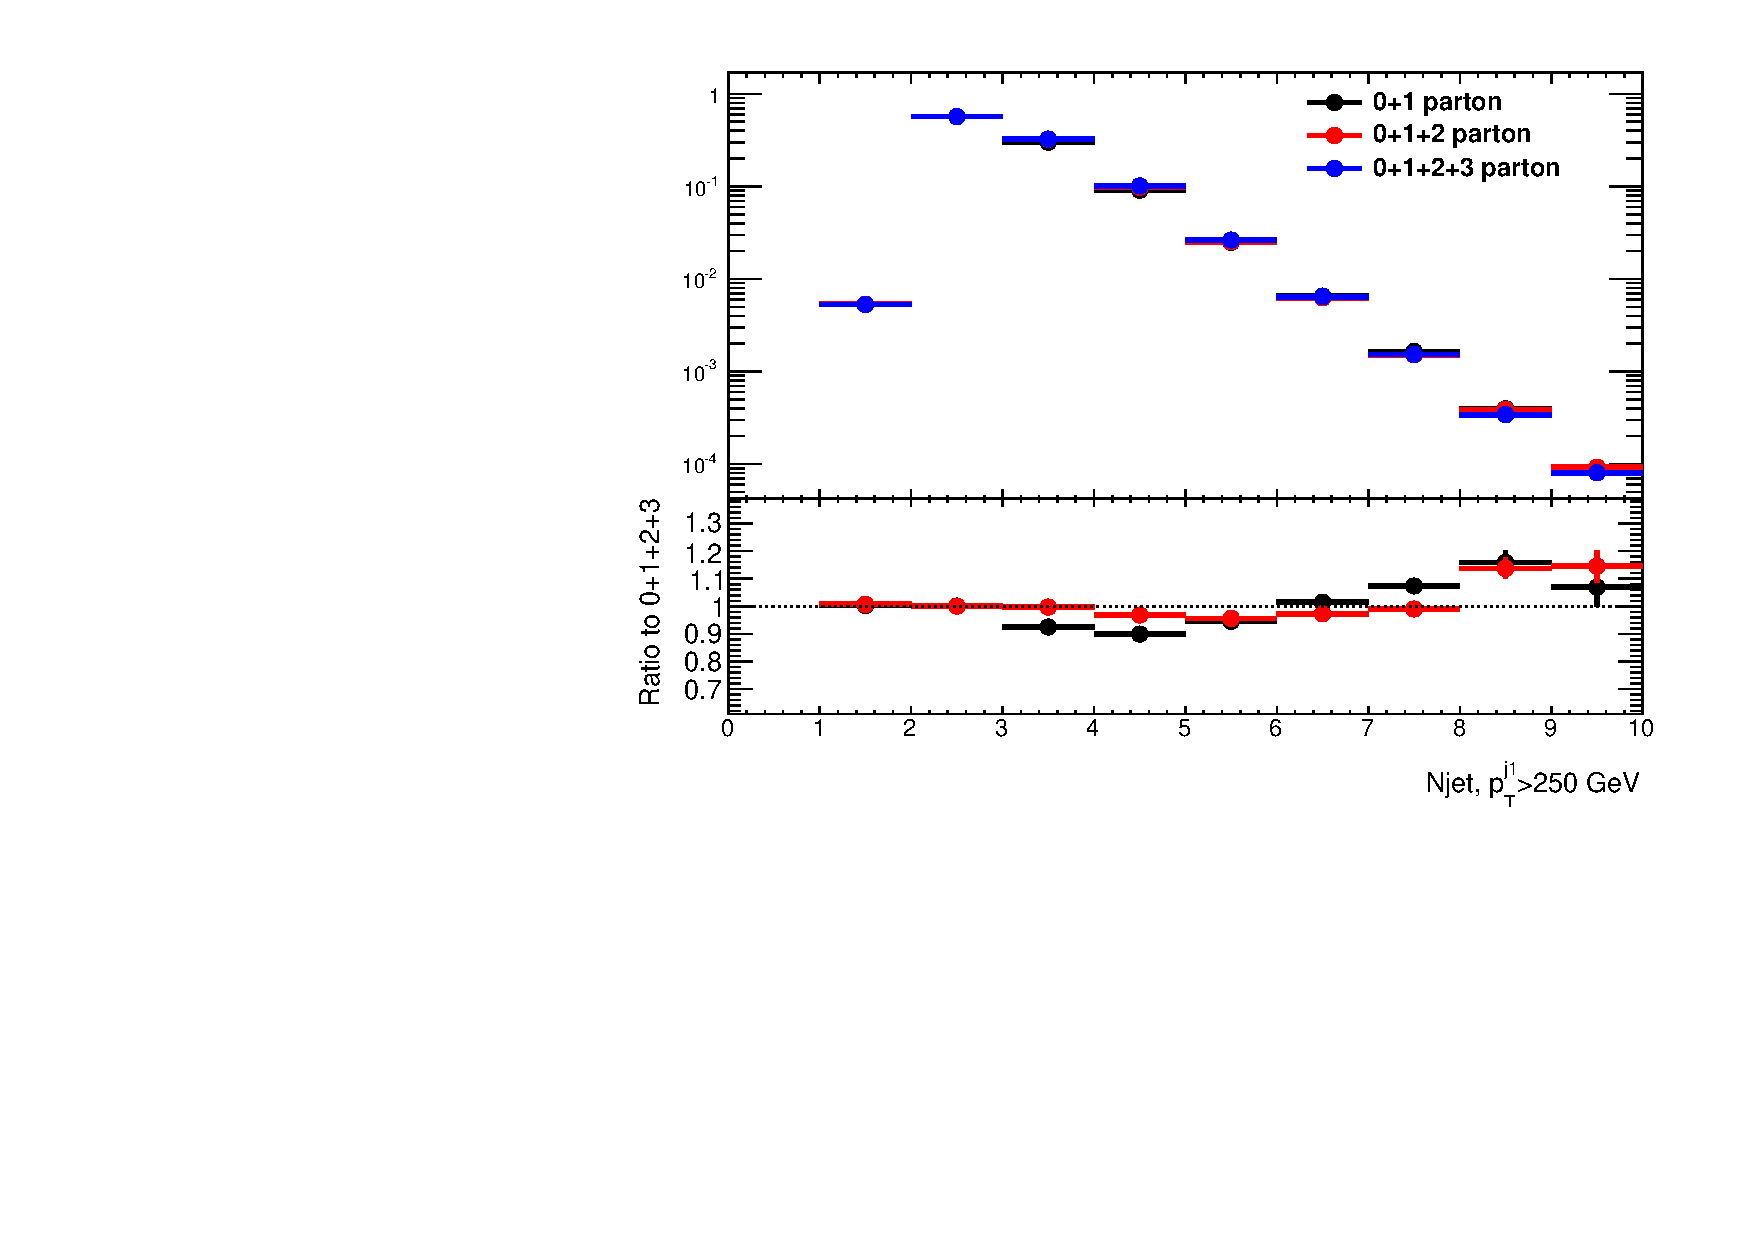
\includegraphics[width=0.8\linewidth]{figures/monojet_appendix/h_njet250.pdf}
%	}
%	\caption{Jet multiplicity distributions for EFT D5 sample with CKKW matching scale at 80 GeV. 0-, 1-, 2- and 3-parton emission cases are generated separatedly and added together by cross sections.}
	\caption{Jet multiplicity distribution for EFT D5 sample with CKKW matching scale at 80 GeV. 0-, 1-, 2- and 3-parton emission cases are generated separatedly and added together by cross sections.}
	\label{fig:RatioKine_D5_2}
\end{figure}

With the ATLAS run-I baseline cut (MET and leading jet $p_{T}$ larger than 250 GeV, less than 4 jets), the 0+1 parton emission has 17.4\% yield less compared to 0+1+2+3 parton emission, while the 0+1+2 has 2.2\% less. With MET$>$400 GeV, 0+1 parton emission has 16.8\% yield less and 0+1+2 parton emission has 2.4\% less compared to 0+1+2+3 parton emission. With MET$>$600 GeV, 0+1 parton emission has 16.5\% yield less and 0+1+2 parton emission has 2.9\% less compared to 0+1+2+3 parton emission. The same numbers hold if a sysmetric cut is added on leading jet transverse momentum.
